%% USPSC-modelo-IFSCe.tex
% ---------------------------------------------------------------
% USPSC: Modelo de Trabalho Acadêmico (tese de doutorado, dissertacao de
% mestrado e trabalhos monograficos em geral) em conformidade com 
% ABNT NBR 14724:2011: Informação e documentação - Trabalhos acadêmicos -
% Apresentação
%----------------------------------------------------------------

\documentclass[
% -- opções da classe memoir --
12pt,		% tamanho da fonte
openright,	% capítulos começam em pág ímpar (insere página vazia caso preciso)
twoside,  % para impressão em anverso (frente) e verso. Oposto a oneside - Nota: utilizar \imprimirfolhaderosto*
a4paper,			% tamanho do papel. 
% -- opções da classe abntex2 --
chapter=TITLE,		% títulos de capítulos convertidos em letras maiúsculas
% -- opções do pacote babel --
english			% idioma
]{USPSC-classe/USPSC}

% ---
% Pacotes matemáticos fundamentais (CORREÇÃO DO ERRO \mathbb)
% ---
\usepackage{amsmath}
\usepackage{amsfonts}
\usepackage{amssymb}

% ---
% Pacotes básicos - Fundamentais 
% ---
\usepackage[T1]{fontenc}		% Seleção de códigos de fonte.
\usepackage[utf8]{inputenc}		% Codificação do documento (conversão automática dos acentos)
\usepackage{lmodern}			% Usa a fonte Latin Modern
\usepackage{lastpage}			% Usado pela Ficha catalográfica
\usepackage{indentfirst}		% Indenta o primeiro parágrafo de cada seção.
\usepackage{color}				% Controle das cores
\usepackage{graphicx}			% Inclusão de gráficos
\usepackage{float} 				% Fixa tabelas e figuras no local exato
\usepackage{chemfig}            % Para escrever reações químicas
\usepackage{chemmacros}         % Para escrever reações químicas
\usepackage{tikz}				% Para escrever reações químicas e outros
\usetikzlibrary{positioning}
\usepackage{pdfpages}
\usepackage{makeidx}            % para gerar índice remissivo
\usepackage{hyphenat}          % Pacote para retirar a hifenizacao DO TEXTO
\usepackage[absolute]{textpos} % Pacote permite o posicionamento do texto
\usepackage{eso-pic}           % Pacote para incluir imagem de fundo
\usepackage{makebox}           % Pacote para criar caixa de texto
\usepackage{braket}
\usepackage{upgreek}

% ---
% Pacotes de citações - Sistema Numérico (IFSC)
% ---
\usepackage{cite}              % agrupa citações numéricas consecutivas
\usepackage[num, abnt-emphasize=bf, abnt-thesis-year=both, abnt-repeated-author-omit=no, abnt-last-names=abnt, abnt-etal-cite=3, abnt-etal-list=3, abnt-etal-text=it, abnt-and-type=e, abnt-doi=doi, abnt-url-package=none, abnt-verbatim-entry=no]{abntex2cite} 
\bibliographystyle{USPSC-classe/abntex2-numeng-USPSC}

% ---
% Configurações de nota de rodapé
% ---
\renewcommand{\thefootnote}{\fnsymbol{footnote}}  %Comando para inserção de símbolos em nota de rodapé
\renewcommand{\footnotesize}{\small} %Comando para diminuir a fonte das notas de rodapé

% ---
% Pacotes adicionais
% ---
\usepackage{lipsum}				% para geração de dummy text
\usepackage{multicol}	% Suporte a mesclagens em colunas
\usepackage{multirow}	% Suporte a mesclagens em linhas
\usepackage{longtable}	% Tabelas com várias páginas
\usepackage{threeparttablex}    % notas no longtable
\usepackage{array}

% ----
% Compatibilização com a ABNT NBR 6023:2018 e 10520:2023
% ----
\usepackage{USPSC-classe/ABNT6023-10520}

% ---
% DADOS INICIAIS
% ---
\siglaunidade{IFSC}
\programa{MFTEe}

% ---
% Configurações de aparência do PDF final
% ---
\definecolor{blue}{RGB}{41,5,195}

\makeatletter
\hypersetup{
	pdftitle={\@title}, 
	pdfauthor={\@author},
	pdfsubject={\imprimirpreambulo},
	pdfcreator={LaTeX with abnTeX2},
	pdfkeywords={abnt}{latex}{abntex}{USPSC}{trabalho acadêmico}, 
	colorlinks=true,       		
	linkcolor=black,          	
	citecolor=black,        		
	filecolor=black,      		
	urlcolor=black,
	bookmarksdepth=4	
}
\makeatother

% O tamanho do parágrafo é dado por:
\setlength{\parindent}{1.3cm}
% Controle do espaçamento entre um parágrafo e outro:
\setlength{\parskip}{0.2cm}  

% compila o sumário e índice
\makeindex

% ----
% Início do documento
% ----
\begin{document}

% Seleciona o idioma do documento como Inglês
\selectlanguage{english}
\frenchspacing 

% --- Formatação dos Títulos
\renewcommand{\ABNTEXchapterfontsize}{\fontsize{12}{12}\bfseries}
\renewcommand{\ABNTEXsectionfontsize}{\fontsize{12}{12}\bfseries}
\renewcommand{\ABNTEXsubsectionfontsize}{\fontsize{12}{12}\normalfont}
\renewcommand{\ABNTEXsubsubsectionfontsize}{\fontsize{12}{12}\normalfont}
\renewcommand{\ABNTEXsubsubsubsectionfontsize}{\fontsize{12}{12}\normalfont}

% ----------------------------------------------------------
% ELEMENTOS PRÉ-TEXTUAIS
% ----------------------------------------------------------
\imprimircapa
\imprimirfolhaderosto*

% Inserir a ficha catalográfica em pdf
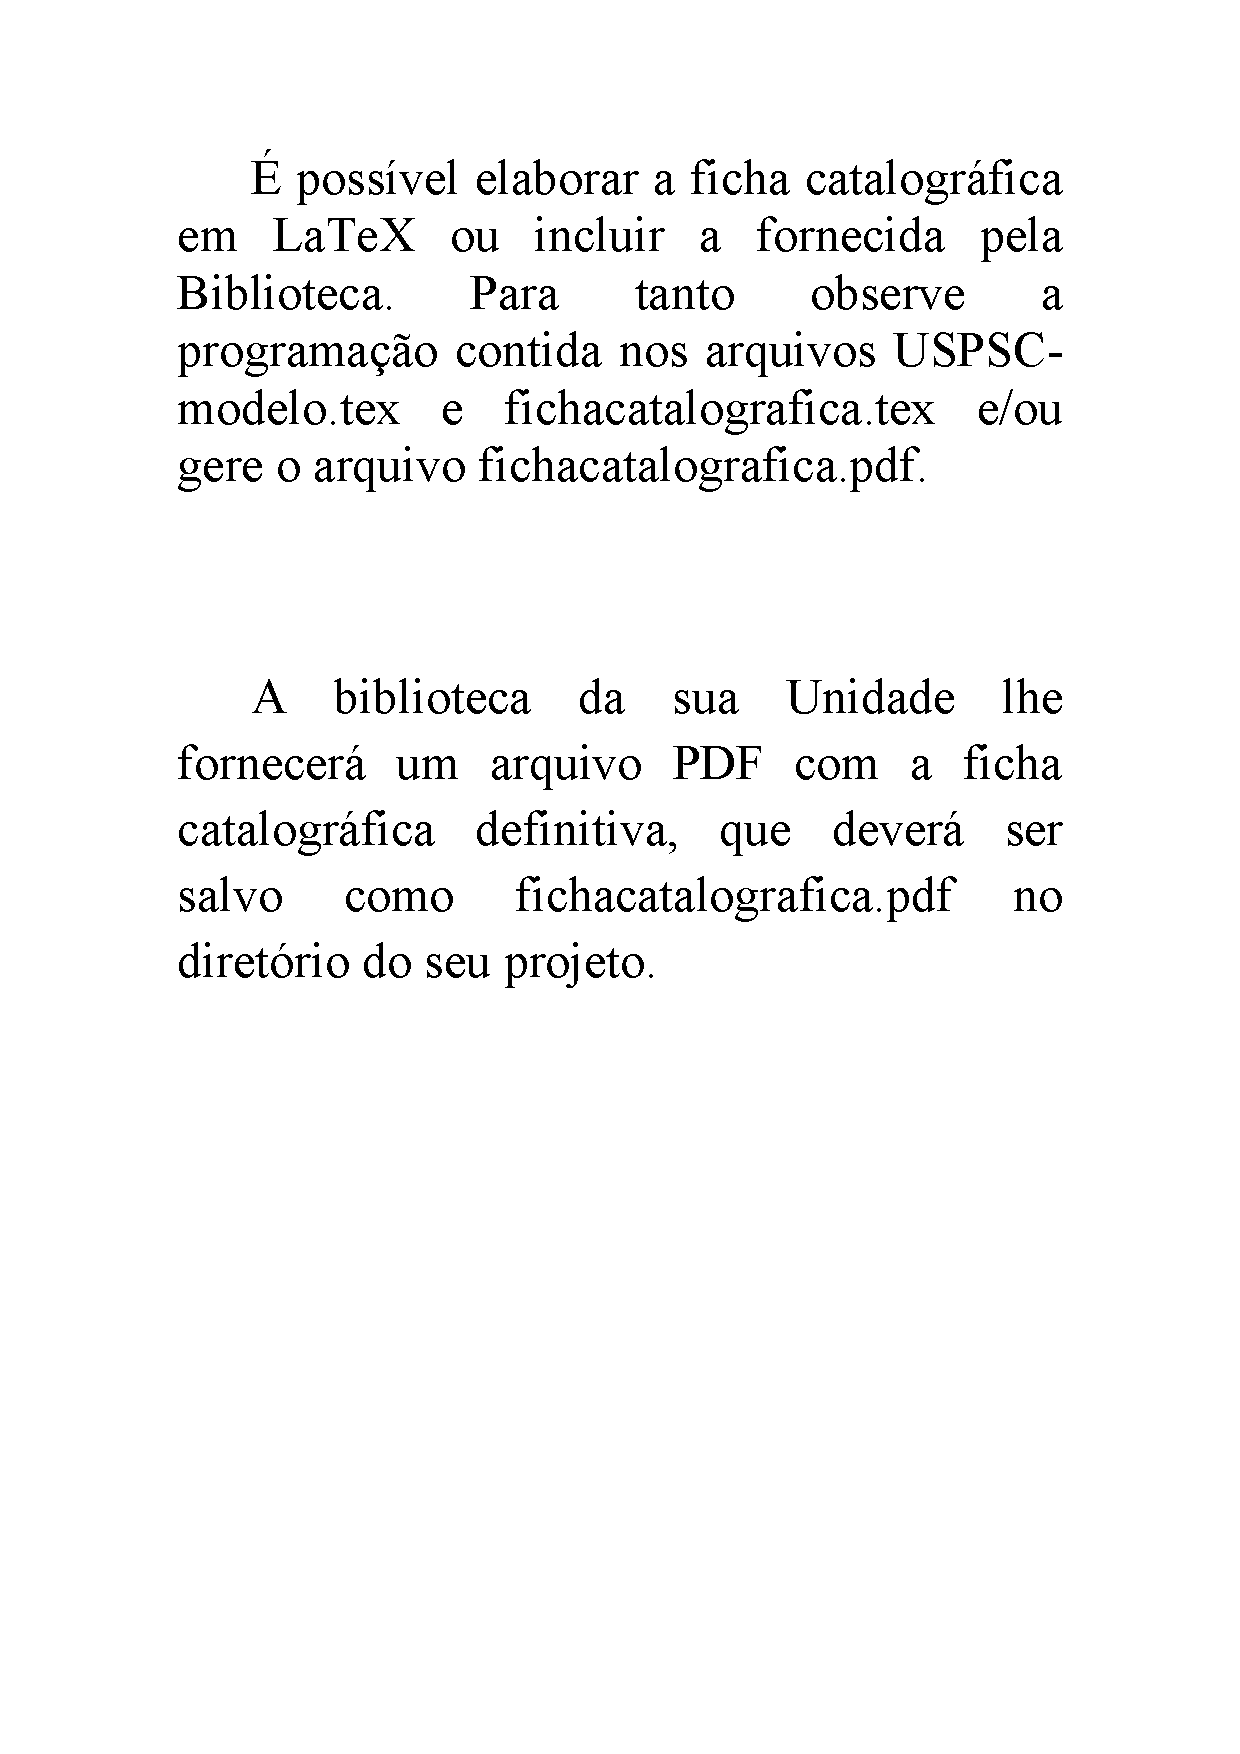
\includepdf{USPSC-TA-PreTextual/USPSC-fichacatalografica.pdf}

% Inserir errata
\include{USPSC-TA-PreTextual/USPSC-Errata}

% Inserir folha de aprovação
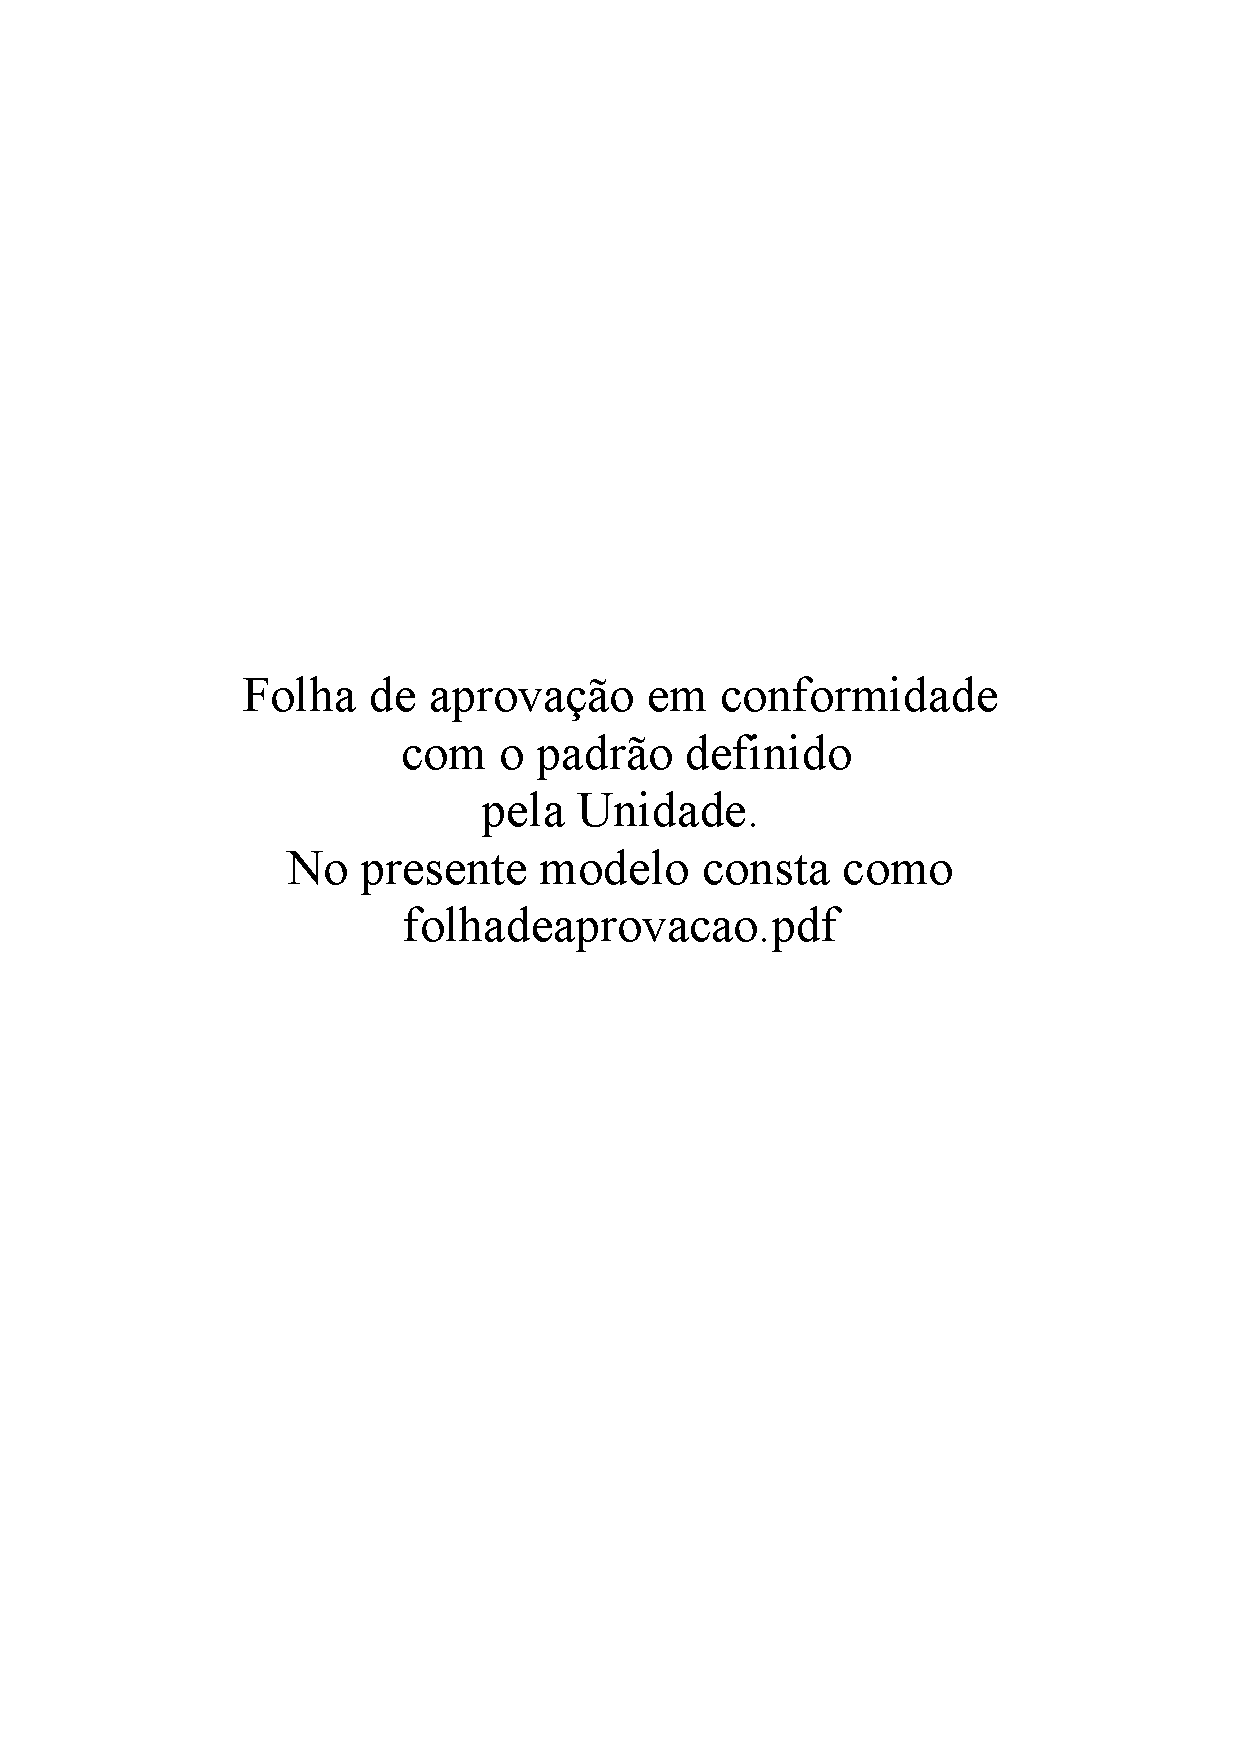
\includepdf{USPSC-TA-PreTextual/USPSC-folhadeaprovacao.pdf}

\includepdf{USPSC-TA-PreTextual/USPSC-PaginaEmBranco.pdf}

% Dedicatória, Agradecimentos e Epígrafe
%% USPSC-Dedicatoria.tex
\begin{dedicatoria}
   \vspace*{\fill}
   \centering
   \noindent
   \textit{Para minha família, meus amigos \\e outros seres vivos que cruzaram meu caminho.} \vspace*{\fill}
\end{dedicatoria}
% ---
%% USPSC-Agradecimentos.tex
\begin{agradecimentos}

	Primeiramente, eu jamais estaria aqui escrevendo estas palavras sem o apoio, cuidado e conhecimento de todos que cruzaram o meu caminho. E honestamente, este espaço é pequeno demais e minhas palavras são imprecisas demais para comunicar o quanto eu tenho a agradecer a todos os seres vivos que fizeram parte desses meus últimos dois anos, mas espero ao menos conseguir transmitir parte da minha gratidão.
	
	Não vejo outra possibilidade senão iniciar os agradecimentos com meus pais. Muito obrigada por serem meu porto seguro em meio ao caos, por sempre me ouvirem e aconselharem a seguir mesmo quando não parecia haver caminhos e por sempre me incentivarem a aprender e crescer. Também não poderia deixar de agradecer toda a alegria, o amor e a torcida da minha família, que cria esse ambiente de pertencimento e acolhimento tão leve e divertido. Gostaria também de dedicar um agradecimento especial às minhas gatas, Morgana e Suri, que, independentemente da distância, sempre melhoram o meu dia. Quero dizer aos meus amigos que a leveza, espontaneidade e aleatoriedades de vocês salvaram muitos dos meus dias. Faço um agradecimento especial aos amigos que fiz em São Carlos, já que minha estadia nessa cidade se tornou muito mais positiva graças à companhia de vocês. Também agradeço de coração ao Lucas pela parceria, incentivo e paciência com meus altos e baixos nessa jornada. Acho essencial que eu agradeça também à minha psicóloga pelo espaço de escuta, suporte e aprendizado.
	
	Além daqueles que me ajudaram a atravessar portas, eu gostaria de agradecer profundamente aqueles que as abriram para mim. Aos meus orientadores, Ivan e Diogo, muito obrigada por me ensinarem tanto sobre física, por me mostrarem como é fazer pesquisa de forma saudável e humana, por criarem espaços acolhedores ao mesmo tempo desafiadores no limite certo para que eu crescesse, e por me apoiarem de todas as formas possíveis. Vocês não só possibilitaram meu mestrado, mas abriram oportunidades para eu transformar em realidade o sonho de ser pesquisadora. Quero também agradecer aos membros do grupo por fazerem da sala 21 um ambiente de trabalho receptivo, divertido e repleto de possibilidades de aprendizado.

    
	
	This study was financed in part by the Coordenação de Aperfeiçoamento de Pessoal de Nível Superior – Brasil (CAPES) – Finance Code 001.
	
\end{agradecimentos}
% ---
%% USPSC-Epigrafe.tex
\begin{epigrafe}
    \vspace*{\fill}
	\begin{flushright}
		\textit{``Eu levarei o Anel, embora eu não saiba o caminho.''\\
		- Frodo Bolseiro (J. R. R. Tolkien, O Senhor dos Anéis)}
	\end{flushright}
\end{epigrafe}
% ---

% Resumos (Como está em inglês, o Abstract vem primeiro)
%% USPSC-Abstract.tex
%\autor{Silva, M. J.}
\begin{resumo}[Abstract]
 \begin{otherlanguage*}{english}
	\begin{flushleft} 
		\setlength{\absparsep}{0pt} % ajusta o espaçamento dos parágrafos do resumo		
 		\SingleSpacing  		\imprimirautorabr~~\textbf{\imprimirtitleabstract}.	\imprimirdata.  \pageref{LastPage} p. 
		%Substitua p. por f. quando utilizar oneside em \documentclass
		%\pageref{LastPage} f.
		\imprimirtipotrabalhoabs~-~\imprimirinstituicao, \imprimirlocal, 	\imprimirdata. 
 	\end{flushleft}
	\OnehalfSpacing 

Understanding how quantum systems equilibrate is a fundamental question with implications for quantum technologies, such as state preparation for quantum computing. However, linear response theory fails to explain the thermal relaxation in the quantum regime and of far-from-equilibrium systems. In this context, recent studies have reported a relaxation asymmetry, where heating is faster than cooling for thermodynamically equidistant initial states, but understanding how quantum resources affect this asymmetry is still an open question. In this work, we investigate the heating and cooling asymmetry in discrete and continuous-variable quantum systems. For the discrete case, we study two interacting qubits coupled to a global bosonic bath, focusing on the effects of initial coherences, steady state correlations generated by the dynamics and local non-Markovianity. For the continuous case, we consider Gaussian states and compare the thermal relaxation asymmetry of displaced and squeezed states. Our results for the discrete case indicate that non-Markovianity may accelerate thermal relaxation, while the initial coherences do not change the equilibration time. In Gaussian systems, applying the displacement operator in the initial states does not affect the asymmetry, but applying the squeezing operator reduces the asymmetry. Additionally, we show an invertion of the asymmetry, making cooling faster than heating, by squeezing the hotter state and displacing the cooler state.

   \vspace{\onelineskip}
 
   \noindent 
   \textbf{Keywords}: asymmetry; relaxation; two-interacting qubits; gaussian systems.
 \end{otherlanguage*}
\end{resumo}

%% USPSC-Resumo.tex
\setlength{\absparsep}{18pt} % ajusta o espaçamento dos parágrafos do resumo		
\begin{resumo}
	\begin{flushleft} 
			\setlength{\absparsep}{0pt} % ajusta o espaçamento da referência	
			\SingleSpacing 
			\imprimirautorabr~~\textbf{\imprimirtituloresumo}.	\imprimirdata. \pageref{LastPage} p. 
			%Substitua p. por f. quando utilizar oneside em \documentclass
			%\pageref{LastPage} f.
			\imprimirtipotrabalho~-~\imprimirinstituicao, \imprimirlocal, \imprimirdata. 
 	\end{flushleft}
\OnehalfSpacing 			

A termodinâmica clássica falha ao tentar explicar a relaxação térmica de sistemas fora do equilíbrio. Estudos recentes mostram uma assimetria nesse regime, onde esquentar é mais rápido do que resfriar estados iniciais termodinâmicamente equidistantes...
 

 \textbf{Palavras-chave}: LaTeX. Classe USPSC. Tese. Dissertação. Trabalho de conclusão de curso (TCC). Relatório.
\end{resumo}

% Listas
\pdfbookmark[0]{\listfigurename}{lof}
\listoffigures*
\cleardoublepage

\pdfbookmark[0]{\listtablename}{lot}
\listoftables*
\cleardoublepage

\pdfbookmark[0]{\listofquadroname}{loq}
\listofquadro*
\cleardoublepage

\include{USPSC-TA-PreTextual/USPSC-AbreviaturasSiglas}
\include{USPSC-TA-PreTextual/USPSC-Simbolos}

% Sumário
\pdfbookmark[0]{\contentsname}{toc}
\tableofcontents*
\cleardoublepage

% ----------------------------------------------------------
% ELEMENTOS TEXTUAIS
% ----------------------------------------------------------
\textual



\chapter{Introduction}\label{cap:intro}

\begin{quote}
    If physical theories were people, thermodynamics would be the village witch. [...] The other theories find her somewhat odd, somehow different in nature from the rest, yet everyone comes to her for advice, and no-one dares to contradict her.\\
    - Goold, Huber, Riera, del Rio, Skrzypczyk (2016)
\end{quote}

The reason everyone comes to this ``village witch" for advise it is her pragmatic approach to nature. Instead of trying to describe microscopic details of a system, she focus on what can be done with its macroscopic resources. This is a consequence of thermodynamics being developed in the context of thermal machines and the goal to achieve efficient exploitation of the natural world. Moreover, this theory development brought fundamental laws regarding energy flow and transformation that have been used in different areas of physics, chemistry, biology, and other sciences. Despite thermodynamics describing macroscopic systems near equilibrium, there is a great effort to extend its concepts to nonequilibrium and quantum regime \cite{goold-2016, vinjanampathy-2016, parrondo-2015, deffner-2019}. This connection of quantum mechanics and thermodynamics can help to understand how quantum systems exchange energy with its surroundings. Because quantum properties can affect transient dynamics, relaxation processes of quantum systems become a non-trivial and timely problem.

Relaxation processes are studied in different areas of physics. Some usual examples are resistor-capacitor circuit, damped harmonic oscillators, dielectric relaxation, and thermal relaxation \cite{moyses-v2, moyses-v3, tipler-v1, tipler-v2, callen-book}. Despite their distinct contexts, this processes are connected in a general way with the question of how systems evolve in time after a perturbation. In this work, we will focus on thermal relaxation processes where we have system interacting with an environment. According to thermodynamics, thermal relaxation is the exchange energy varying the system's temperature until it reaches a steady state. If the system is in a thermodynamic state near equilibrium, this evolution can be described using linear response theory, such as Onsager-Casemir and Kubo-Yokota-Nakajima laws \cite{lapolla-2020}. In this regime, the mean behaviour of statistical fluctuations is the same as the macroscopic system, being valid the assumption that the dynamics is memoryless and symmetric. Considering a thermal relaxation process, symmetry means that heating up or cooling down the system will take the same amount of time and follow the same thermodynamic trajectory \cite{ibanez-2024, lapolla-2020, seifert-2012, groot-2013}.

However, thermal relaxation symmetry can break for systems initially far from equilibrium and quantum systems, where linear response theory fails. One example of thermal relaxation asymmetry is the Mpemba effect. First observations of the Mpemba effect were that a hotter system (such as water) would cool down faster than a colder one \cite{mpemba-1969, kell-1969, teza-2026}. There is also the inverse Mpemba effect that occurs in heating processes instead of cooling \cite{teza-2026}. In general terms, Mpemba-like effects consist of a system further from equilibrium relaxing faster than another system closer to equilibrium. In this respect, Mpemba effects have been explored in the quantum regime \cite{krissia-2024, summer-2026, calabrese-2026, ares-2025, teza-2026}, such as the ergotropic Mpemba effect, where it was found that squeezed states relax faster than displaced states even when the ergotropy of squeezing is bigger (which means it is further from equilibrium) \cite{medina-2025}. Another relaxation asymmetry that emerges in the far-from-equilibrium regime is the heating-cooling asymmetry. Recent experiments using Brownian motion showed that heating is faster than cooling \cite{lapolla-2020, ibanez-2024, dieball-2023}. This was also observed to happen in quantum systems, such as a qubit, a quantum harmonic oscillator, and in quantum Brownian motion \cite{tejero-2025, manikandan-2021}. However, this behaviour is not universal, as it is possible to observe cooling relaxing faster than heating depending on the system's characteristics, for example, energy gap or degeneracy in systems with more than two levels \cite{vu-2021, bravetti-2025, teza-2026}. In addition, it is interesting that this heating-cooling asymmetry can also appear when comparing the usual Mpemba effect (cooling) with the inverse Mpemba effect (heating) \cite{teza-2026}.

A better understanding of relaxation asymmetries can be useful for state preparation \cite{verstraete-2009, harrington-2022}, optimal transport \cite{walker-2023}, heat engines \cite{liu-2024, liu-2026}, and other applications \cite{teza-2026}. For this purpose, beyond phenomenological characterisation, it is fundamental to study the physical mechanisms generating the asymmetries. To do this, previous studies developed an approach named thermal kinematics using the combination of stochastic thermodynamics and information geometry \cite{ito-2018, dechant-2020,ibanez-2024}. In thermal kinematics, thermodynamic states can be interpreted as points in a manifold, and we can define a distance between different states. As the system evolves in time, it will have a velocity and follow a thermodynamic trajectory in this manifold. Using this approach, Ref. \cite{ibanez-2024} proved that heating and cooling systems far from equilibrium follow distinct thermodynamic trajectories. Later, thermal kinematics was extended to the quantum regime, where this same result was obtained \cite{tejero-2025}. From a thermodynamic perspective, previous works showed that heating-cooling asymmetry can be explained by entropy production, in which heating is faster because it has a higher entropy production than cooling can dissipate heat \cite{tejero-misc-2025}. In addition to these works, understanding the consequences of quantumness in the heating-cooling asymmetry is still an open question. It is known that quantum correlations have consequences in thermodynamic processes, such as the case of anomalous heat exchange \cite{amikam-2020} and non-classical work extraction \cite{paternostro-2020, campaioli-2024}. Additionally, in the context of thermal relaxation, coherence in a qubit was shown to delay equilibration \cite{krissia-2024}. Therefore, the main question of this work is what quantumness do with the heating-cooling asymmetry.

There is a variety of systems and models we can use to explore this question. By observing different physical theories and phenomena, we see that discrete and continuous-variable models bring complementary explanations of nature. In addition, finding the analogous phenomena in both types of systems also enriches potential technological applications. Motivated by these considerations, this work explores the thermal relaxation asymmetry in both discrete and continuous-variable quantum systems. For the discrete case, we will focus on the thermal relaxation of two interacting qubits coupled to a global bath. Despite the variety of quantum properties we could investigate, we will focus only on quantum coherence and entanglement for this model. For the continuous-variable case, we focus on Gaussian states due to their relevance in quantum theory and experimental accessibility \cite{adesso-2016, stefanini-2026}.

In this work, we start discussing how open quantum systems evolve in time in Chap. \ref{cap:oqs}, where we derive the Lindblad master equation and present the thermalization dynamics called Davies map, that will be used in our results. Then, in Chap. \ref{cap:thermo}, we extend some thermodynamics concepts and quantities to the quantum regime, such as entropy and free energy. This chapter also introduces the thermal kinematics approach for both classical and quantum regime. Chap. \ref{cap:results-discrete} starts presenting the quantum properties that we will study for the discrete case. Next, we show our results for the heating-cooling asymmetry in two-interacting qubits model, where we investigate the effects of initial global coherences and correlations generated between the qubits during the dynamics. In Chap. \ref{cap:results-continuous}, we present the continuous-variable systems we will study that are Gaussian states. After showing the basic concepts, we discuss the thermalization of Gaussian states and reformulate the thermal kinematics approach for this case. With this, we show the results for the heating-cooling asymmetry in a thermal state, a displaced state, a squeezed state, and we show one way to invert the asymmetry. We end this work by summarising our results and suggesting future directions on this research topic.



\chapter{Introduction to Open Quantum Systems Theory}\label{cap:oqs}

This chapter introduces how quantum systems evolve in time. We begin discussing the unitary evolution of closed quantum systems in Sec. \ref{sec:close}. However, this description cannot be applied to open quantum systems. A solution for this is presented in Sec. \ref{sec:open}, where we present a Markovian master equation and specify its form to describe a thermalisation process. The content of this chapter are based on Refs. \cite{petruccione-book, scully-book, rivas-2010}.



\section{Dynamics of Close Quantum Systems} \label{sec:close}
%Close Quantum Systems Evolution and motivation for OQS
% 1. eq de schrodinger + sistemas fechados ideais
% 2. estados puros vs mistura estatistica = introduzir density matrices
% 3. Liouville-von Neumann
% 4. por que falha para sistemas abertos? perda de unitariedade

Quantum mechanics was initially formulated for isolated systems, whose physical states are represented as a normalised vector $\ket{\psi}$ in the Hilbert space $\mathcal{H}$. This representation contains all the information about the physical state, called a pure state. However, another mathematically equivalent formulation is more convenient for describing quantum systems whose states are not fully known. In these cases, it is only possible to assign a probability $p_i$ of the system existing in the state $\ket{\psi_i}$, which is encapsulated in the density operator,
\begin{equation}
    \hat{\rho} = \sum_i p_i \ket{\psi_i} \bra{\psi_i}.
\end{equation}

\noindent The pure state is a special case in the density operator notation, where it is written as $\hat{\rho} = \ket{\psi}\bra{\psi}$. The density operator (also called density matrix) must satisfy the following conditions: (1) the sum of all $p_i$ is equal to one, which is equivalent to $\text{Tr}[\hat{\rho}] = 1$, and (2) it is positive semi-definite, which means all $\hat{\rho}$ eigenvalues are $\lambda_k \geq 0$.

More than describing physical states, quantum mechanics explains how quantum systems evolve in time. For closed quantum systems, the time evolution is given by the Schrödinger equation,
\begin{equation}
    i \hbar \frac{d}{dt} \ket{\psi (t)} = \hat{H}(t) \ket{\psi (t)},
\end{equation}
\noindent where $\hat{H}(t)$ is the system's Hamiltonian and Planck's constant will be $\hbar = 1$ from now on. This equation can be translated into the density matrices notation as the Liouville-von Neumann equation,
\begin{equation}
    \frac{d}{dt} \hat{\rho}(t) = - i [\hat{H}(t), \hat{\rho} (t)].
\end{equation}

\noindent Its solution describes the unitary evolution of an initial state $\hat{\rho}(0)$ as
\begin{equation}
    \hat{\rho}(t) = U(t) \hat{\rho} (0) U^\dagger (t),
\end{equation}

\noindent where $U(t)$ is a unitary operator with properties $U^{-1} = U^\dagger$ and $U U^\dagger = \mathbb{I}$, in which $\mathbb{I}$ is the identity matrix. Unitary dynamics conserve the total probability, which makes sense as an isolated system cannot lose any information. A consequence of preserving the information is that the dynamics are time-reversible.

Even though all this formalism describes a variety of quantum phenomena, it is an idealisation because every physical system interacts with others. So, let's take a step forward and consider a quantum system ($S$) interacting with another system called the environment ($E$). Together, they form a closed quantum system that evolves in time by the unitary dynamics described before. The total system ($S+E$) is defined by the Hamiltonian
\begin{equation}
    \hat{H}_{SE} = \hat{H}_S \otimes \mathbb{I}_E + \mathbb{I}_S \otimes \hat{H}_E + \hat{H}_I,
\end{equation}

\noindent where $\hat{H}_S$ is the system's Hamiltonian, $\hat{H}_E$ is the environment's Hamiltonian, and $\hat{H}_I$ describes the system-environment interaction. Some characteristics of the environment are that it does not evolve with time and is usually considered to have infinite degrees of freedom, over which we cannot access information or have control. As a result, the system $S$ is the only part we can manipulate, being the focus of our studies. However, because the system $S$ exchanges information with the environment, it does not have a unitary dynamics in general. This is what we call an open quantum system, illustrated in Fig. \ref{fig:oqs-scheme}, whose dynamics will be introduced in the next section.

\begin{figure}[b!]
    \centering
    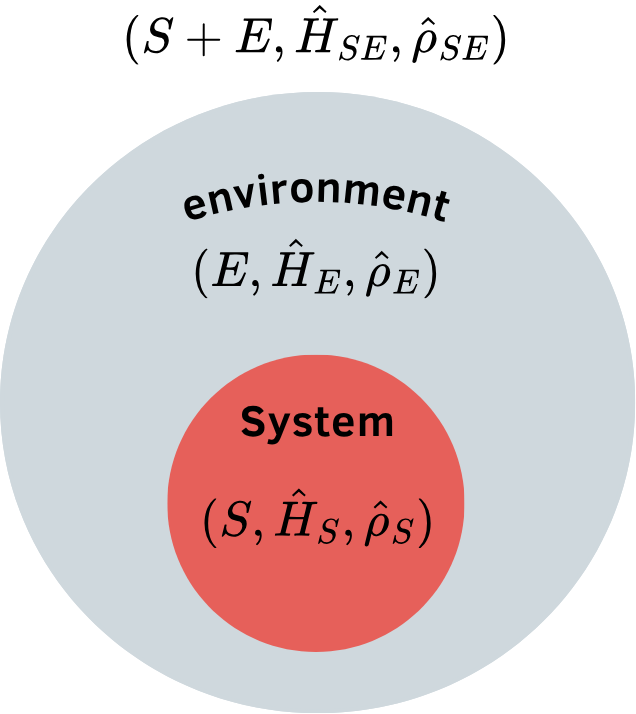
\includegraphics[width=0.35\linewidth]{Images/open-systems-scheme.png}
    \caption{Scheme of an open quantum system.}
    \label{fig:oqs-scheme}
\end{figure}


\section{Dynamics of Open Quantum Systems} \label{sec:open}
%Derivation of Master Equations (Markovian approximation and weak-coupling)
%Davies Map

In this section, we discuss the fundamental steps to obtain the Gorini-Kossakowski-Sudarshan-Lindblad (GKSL) master equation, also called the Lindblad master equation for short. Let's begin with the time evolution of the total system ($S+E$). We know it is unitary, meaning that the Liouville-von Neumann equation can be used. However, we do not have access to all the information in the environment, and including its dynamics in the calculation can be overwhelming. Fortunately, it is possible to make some approximations to describe the system's dynamics, taking into account environmental effects, without needing to deal with the environment's time evolution. These approximations become a bit easier in the interaction picture, where both states and operators change with time. Up to this point, we have used the Schrödinger picture, in which the state evolves with time while the operators remain unchanged. To convert from the Schrödinger picture to the interaction picture, we split the total Hamiltonian as $H_{SE} = H_0 + H_I$ with $H_0 = \hat{H}_S \otimes \mathbb{I}_E + \mathbb{I}_S \otimes \hat{H}_E$, and the time evolution of an operator $\hat{O}$ becomes $\hat{O}(t) = e^{iH_0 t} \hat{O} e^{-iH_0 t}$. As a result, the Liouville-von Neumann equation describing the total system-environment dynamics becomes
\begin{equation}
    \frac{d}{dt} \hat{\rho}_{SE}(t) = -i [\hat{H}_I (t), \hat{\rho}_{SE}(t)].
    \label{eq:neumann-diferencial}
\end{equation}

\noindent We can integrate this equation and substitute into itself, obtaining
\begin{equation}
    \frac{d}{dt}\hat{\rho}_{SE}(t) = -i [\hat{H}_I(t), \hat{\rho}_{SE}(0)] - \int_{0}^{t} ds [\hat{H}_I(t), [\hat{H}_I(s), \hat{\rho}_{SE}(s)]].
\end{equation}

\noindent Because we are only interested in the system's dynamics, we can erase the environment by taking the partial trace. All this algebra still has not solved the problem with environmental dynamics, so our next steps are making approximations. First, we will consider a weak system-environment interaction, allowing us to use the Born approximation, $\hat{\rho}_{SE} (t) \approx \hat{\rho}_S (t) \otimes \hat{\rho}_E$. An interesting consequence of using the weak coupling is that the environment is essentially unaffected by the system $S$, so it can be considered memoryless, allowing us to apply the Markov approximation. In other words, the time the environment takes to erase the system's perturbation is much shorter than the relaxation time, which is equivalent to extending $t \rightarrow \infty$. By using the Markovian approximation, the system's time evolution does not depend on its past states, which means $\rho_S(s) = \rho_S(t)$. After all these approximations, we find the Redfield equation,
\begin{equation}
    \frac{d}{dt} \hat{\rho}_{S}(t) = -i \text{Tr}_E[\hat{H}_I(t), \hat{\rho}_S (0) \otimes \hat{\rho}_E] - \text{Tr}_E\int_{0}^{\infty} ds [\hat{H}_I(t), [\hat{H}_I(s), \hat{\rho}_S (t) \otimes \hat{\rho}_E]].
    \label{eq:redfield}
\end{equation}

\noindent In most cases, the mean of environmental fluctuations is zero, which makes the first term zero. So, we will focus our analysis on the second term.

Although Eq. \eqref{eq:redfield} can describe the relaxation of open quantum systems, it does not guarantee the positivity of probabilities, which can lead to unphysical results. Then, a solution is to use one last approximation: the rotating wave approximation (RWA). In this section, we will use a simpler scenario to make the RWA, but the general case can be found in \cite{petruccione-book}. Let's consider that a perturbation of the bath results in a single effect on the system, that is, no multiple transitions can occur simultaneously in the system. So, the interaction Hamiltonian in the Schrödinger picture can be decomposed into two Hermitian operators as
\begin{equation}
    \hat{H}_I = \hat{A} \otimes \hat{B},
    \label{eq:HI-AkBk}
\end{equation}

\noindent The next step is to write $\hat{A}$ in terms of the eigenstates of the system's Hamiltonian, $\hat{H}_S \ket{n} = \lambda_n \ket{n}$. To make the RWA, we will separate this operator as $\hat{A} = \sum_\omega \hat{A} (\omega)$, where
\begin{equation}
    \hat{A} (\omega) = \sum_{\substack{n,m \\ \omega = \lambda_m - \lambda_n}} \ket{n}\bra{n} \hat{A} \ket{m}\bra{m}
    \label{eq:Ak-w}
\end{equation}

\noindent is summing over all combinations of states that have frequency $\omega$. In the interaction picture, this Hamiltonian becomes
\begin{equation}
    \hat{H}_I (t) = \sum_{\omega} e^{-i\omega t} \hat{A} (\omega) \otimes \hat{B} (t) = \sum_{\omega'} e^{i\omega' t} \hat{A}^\dagger (\omega') \otimes \hat{B}^\dagger (t).
\end{equation}

\noindent The last equality came from using the property $A (\omega) = A^\dagger (-\omega)$ and $\omega' = -\omega$. With this decomposition of the interaction Hamiltonian, we use $s \rightarrow t-s$ and define
\begin{align}
    &\hat{H}_I (t-s) = \sum_{\omega} e^{-i\omega (t-s)} \hat{A} (\omega) \otimes \hat{B} (t-s),\\
    &\hat{H}_I (t) = \sum_{\omega'} e^{i\omega' t} \hat{A}^\dagger (\omega') \otimes \hat{B}^\dagger (t),
\end{align}

\noindent to rewrite Eq. \eqref{eq:redfield} as
\begin{equation}
    \begin{split}
        \frac{d}{dt} \hat{\rho}_{S}(t) &= - \text{Tr}_E\int_{0}^{\infty} ds [\hat{H}_I(t), [\hat{H}_I(t-s), \hat{\rho}_S (t) \otimes \hat{\rho}_E]]\\
        &= \sum_{\omega, \omega'} e^{i (\omega' - \omega)t} \Gamma (\omega) (\hat{A} (\omega) \hat{\rho}_S (t) \hat{A}^\dagger (\omega') - \hat{A}^\dagger (\omega') \hat{A} (\omega) \hat{\rho}_S (t)) + \text{h.c},
    \end{split}
\end{equation}

\noindent where
\begin{equation}
    \Gamma (\omega) = \int_0^{\infty} ds e^{i\omega s} \braket{\hat{B}^\dagger (t) \hat{B} (t-s)}_E,
\end{equation}

\noindent with $\braket{\hat{B}^\dagger (s) \hat{B} (0)}_E = \text{Tr}[\hat{B}^\dagger (s) \hat{B} (0) \hat{\rho}_E]$ being the correlation functions of the bath. The rotating wave approximation imposes that the terms with $\omega \neq \omega'$ oscillate so fast that they do not affect the relaxation process. As a result, only the cases of resonance ($\omega = \omega'$) contribute to the equation. Thus we have
\begin{equation}
    \frac{d}{dt} \hat{\rho}_{S}(t) = \sum_{\omega} \Gamma (\omega) (\hat{A} (\omega) \hat{\rho}_S (t) \hat{A}^\dagger (\omega) - \hat{A}^\dagger (\omega) \hat{A} (\omega) \hat{\rho}_S (t)) + \text{h.c}.
\end{equation}

\noindent One last step to obtain the usual form of the Lindblad master equation is to separate $\Gamma(\omega)$ into its real and imaginary parts as
\begin{equation}
    \Gamma (\omega) = \frac{1}{2} \gamma (\omega) + i S (\omega),
    \label{eq:Gamma-coef}
\end{equation}

\noindent where the transition rate is
\begin{equation}
    \gamma (\omega) = \int_{-\infty}^{\infty} ds e^{i \omega s} \braket{\hat{B}^\dagger (s) \hat{B} (0)}_E,
    \label{eq:gamma-coef}
\end{equation}

\noindent and $S (\omega)$ produce slight changes on the system's energy levels, which are included in the Lamb shift Hamiltonian 
\begin{equation}
    \hat{H}_{LS} = \sum_\omega S (\omega) \hat{A}^\dagger (\omega) \hat{A} (\omega).
    \label{eq:hamiltonian-lamb-shift}
\end{equation}

\noindent As a result, the Lindblad master equation in the interaction picture has the form
\begin{equation}
    \frac{d}{dt} \hat{\rho}_{S}(t) = -i [\hat{H}_{LS}, \hat{\rho}_S (t)] + \mathcal{D}(\hat{\rho}_S(t)),
    \label{eq:lindblad-interaction}
\end{equation}

\noindent with the dissipator being
\begin{equation}
    \mathcal{D}(\hat{\rho}_S) = \sum_\omega \gamma (\omega) \left(\hat{A} (\omega) \hat{\rho}_S \hat{A}^\dagger (\omega) - \frac{1}{2} \{ \hat{A}^\dagger (\omega) \hat{A} (\omega) , \hat{\rho}_S \} \right),
    \label{eq:dissipator}
\end{equation}

\noindent where $\hat{A} (\omega)$ are usually called jump operators. In the Schrödinger picture, the Lindblad master equation becomes
\begin{equation}
    \frac{d}{dt} \hat{\rho}_{S}(t) = -i [\hat{H}_S + \hat{H}_{LS}, \hat{\rho}_S (t)] + \mathcal{D}(\hat{\rho}_S(t)),
    \label{eq:lindblad}
\end{equation}

\noindent where the jump operators remain the same. It is very common to neglect the Lamb shift Hamiltonian, because it only adds a constant to the expression, without changing the physics of the system. That said, from now on, we will use only the $\hat{H}_S$ in our Lindblad master equation.



%%%%%%%%%%%%%%%%%%%%%%%%%%%%%%%%%%%%%%%%%%%%
\subsection{Davies Maps}\label{sec:davies-maps}

An important class of Lindblad master equations is the Davies maps, which generate the thermalisation of a quantum system weakly coupled to a thermal bath at inverse temperature $\beta$ \cite{davies-1979}. This relaxation process always results in thermal states, which means the Davies maps' steady state is always a Gibbs state of the form
\begin{equation}
    \hat{\rho}_{ss} = e^{-\beta \hat{H}_S}/\mathcal{Z}_S,
\end{equation}

\noindent where $\mathcal{Z}_S = \text{Tr}[\exp(-\beta \hat{H}_S)]$ is the partition function. For this to be true, the transition rates $\gamma (\omega)$ must obey the detailed balance condition,
\begin{equation}
    \gamma(-\omega) = \gamma (\omega) e^{-\beta \omega}.
    \label{eq:detailed-balance}
\end{equation}

\noindent Given these conditions, the jump operators of the Davies map have a specific format. Let's rewrite the dissipator (Eq. \eqref{eq:dissipator}) as
\begin{equation}
    \mathcal{D}(\hat{\rho}_S) = \sum_\omega \hat{L}_\omega \hat{\rho}_S \hat{L}_\omega^\dagger - \frac{1}{2} \{ \hat{L}_\omega^\dagger \hat{L}_\omega , \hat{\rho}_S \},
    \label{eq:dissipator-L}
\end{equation}

\noindent defining the jump operators as $\hat{L}_\omega = \sqrt{\gamma (\omega)} \hat{A}(\omega)$. To compute the transition rate ($\gamma (\omega)$), according to Eq. \eqref{eq:gamma-coef}, we need to use that our environment is a thermal bath. The thermal bath can be described by a set of infinite independent harmonic oscillators, $\hat{H}_E = \sum_k \omega_k \hat{b}_k^\dagger \hat{b}_k$, where $\omega_k$ is the frequency of the $k$-mode, and $\hat{b}_k$ and $\hat{b}_k^\dagger$ are the annihilation and creation operators of the $k$-mode. That said, the hermitian operator from Eq. \eqref{eq:HI-AkBk} $\hat{B} = \sum_k (g_k \hat{b}_k^\dagger + g_k^* \hat{b}_k)$ in the interaction picture is
\begin{equation}
    \hat{B} (s) = \sum_k (g_k \hat{b}_k^\dagger e^{i \omega_k s} + g_k^* \hat{b}_k e^{-i \omega_k s}),
\end{equation}

\noindent with $g_k$ being the system-environment coupling parameter. The density matrix of the thermal bath is 
\begin{equation}
    \hat{\rho}_E = \prod_i (1- e^{-\beta \omega_i}) e^{-\beta \omega_i \hat{b}_i^\dagger \hat{b}_i},
\end{equation}

\noindent with which we can compute the correlation functions, obtaining
\begin{equation}
    \braket{\hat{B}^\dagger (s) \hat{B} (0)}_E = \sum_k |g_k|^2 ( e^{-i \omega_k s} (\bar{n}(\omega_k) +1) + e^{i \omega_k s} \bar{n}(\omega_k)),
\end{equation}

\noindent where $\bar{n}(\omega_k) = (e^{\beta \omega_k} -1)^{-1}$ is the Bose-Einstein distribution. Then, we find the transition rates by solving the integral in Eq. \eqref{eq:gamma-coef}, resulting in
\begin{align}
    &\gamma (-\omega) = 2\pi \sum_k |g_k|^2 \bar{n}(\omega_k) \delta(\omega - \omega_k)\\
    &\gamma (+\omega) = 2\pi \sum_k |g_k|^2 (\bar{n}(\omega_k) + 1) \delta(\omega - \omega_k).
\end{align}

\noindent Assuming that the infinite harmonic oscillators of the bath have close frequencies, we can convert from discrete to continuum space by changing the sum to an integral in $\omega$, $g_k$ to a function $g(\omega)$ and including the density function of the bath's states $d(\omega)$. The solution of this new integral gives transition rates that respect the detailed balance (Eq. \eqref{eq:detailed-balance}),
\begin{align}
    &\gamma (-\omega) = \Gamma (\omega) \bar{n}(\omega),\\
    &\gamma (+\omega) = \Gamma (\omega) (\bar{n}(\omega) + 1),
\end{align}

\noindent where $\Gamma (\omega) = 2\pi d(\omega) |g(\omega)|^2$. Considering a homogeneous bath and the same coupling for all $k$-modes, $\Gamma$ becomes a constant. Also, because we have two frequencies, we solve the sum in $\omega$ from the Eq. \eqref{eq:dissipator-L}, obtaining the following Lindblad equation for the Davies maps,
\begin{equation}
    \frac{d}{dt}\hat{\rho}_S (t) = -i [\hat{H}_S, \hat{\rho}_S (t)] + \mathcal{D}^{-} (\hat{\rho}_S) + \mathcal{D}^{+} (\hat{\rho}_S),
    \label{eq:lindblad-davies}
\end{equation}

\noindent where each dissipator's jump operator is
\begin{align}
    &L_\omega^{+} = \sqrt{\Gamma (\bar{n}(\omega)+1)} \hat{A}(\omega),\\
    &L_\omega^{-} = \sqrt{\Gamma \bar{n}(\omega)} \hat{A}(\omega),
\end{align}

After discussing some of the open quantum systems theory, it is always helpful to solve an example. Below, we will solve the thermalisation of a single-mode harmonic oscillator, whose solution will be used later in this work's results.

\subsubsection{Example: single-mode harmonic oscillator coupled to a thermal bath}\label{sec:example}

Consider the system is a single-mode harmonic oscillator $\hat{H}_S = \omega_0 \hat{a}^\dagger \hat{a}$ with $\hat{a}$ and $\hat{a}^\dagger$ being its annihilation and creation operators, respectively. As we discussed before, this system is coupled to a thermal bath of temperature $\beta$, and the relaxation process is described by Eq. \eqref{eq:lindblad-davies}.

Let's find out the jump operators of this case. Usually, the Hermitian operator of the interaction acting on the system subspace is defined as $\hat{A} = \hat{a} + \hat{a}^\dagger$. To decompose $\hat{A}$ into $\hat{A}(\omega)$, we must find out the eigenstates of $\hat{H}_S$ and the frequencies at which this interaction operator makes transitions in our systems. The eigenstates of the harmonic oscillator are Fock states, $\hat{H}_S \ket{n} = \lambda_n \ket{n}$ with $\lambda_n = n \omega_0$. For these states, the creation operator raises one energy level ($\hat{a}^\dagger \ket{n} = \sqrt{n+1} \ket{n+1}$) and the annihilation operator lowers one energy level ($\hat{a} \ket{n} = \sqrt{n} \ket{n-1}$) Using that the energy difference is given by $\lambda_m - \lambda_n = (m - n) \omega_0$, the possible transition frequencies are $+\omega_0$ or $-\omega_0$. Then, the terms of the decomposition of $\hat{A}$ according to Eq. \eqref{eq:Ak-w} becomes
\begin{align}
    &\hat{A}(+\omega_0) = \sum_{m} \ket{m-1}\bra{m-1} \hat{A} \ket{m}\bra{m} = \hat{a},\\
    &\hat{A}(-\omega_0) = \sum_{m} \ket{m+1}\bra{m+1} \hat{A} \ket{m}\bra{m} = \hat{a}^\dagger.
\end{align}

\noindent As a result, the jump operators of this thermal relaxation are
\begin{align}
    &L_\omega^{+} = \sqrt{\Gamma (\bar{n}(\omega)+1)} \hat{a},\\
    &L_\omega^{-} = \sqrt{\Gamma \bar{n}(\omega)} \hat{a}^\dagger.
\end{align}

\noindent This example is fundamentally related to Gaussian states, which will be introduced in Sec. \ref{sec:gaussian}. In Sec. \ref{sec:result-gaussian}, we will analytically solve this master equation.


\chapter{Quantum Thermodynamics} \label{cap:thermo}


\section{Quantum Correlations} \label{sec:correlations}

\section{Thermodynamic variables in classical and quantum regime} \label{sec:thermo-variables}

\section{Equilibrium and Nonequilibrium States} \label{sec:equilibrium}

\section{Relaxation, Entropy Production and Irreversibility} \label{sec:relaxation}

\subsection{Non-Markovianity}
%Non-Markovianity
%   Definition
%   Quantifying non-Markovianity
%   Relation with entropy production

Up to this point, we have discussed how to describe Markovian relaxation of open quantum systems. However, the Born-Markov approximation is not valid for many processes of open quantum systems, for example, with strong coupling \textcolor{red}{cite}, structured reservoirs \cite{brito-2015, popovic-2018}, or large initial system-environment correlations \textcolor{red}{cite}. In these cases, memory effects become relevant for the time evolution of the system, a phenomenon known as non-Markovian dynamics. There are a variety of ways to measure and witness non-Markovianity. For example, in information theory, integrating the trace distance in time can quantify the information backflow \cite{breuer-2015}. Another example is analysing the divisibility of the maps that generate the system's dynamics \cite{rivas-2010}. In this work, we are interested in a witness of non-Markovianity that connects the information and thermodynamic analysis: the entropy production \cite{popovic-2018, marcantoni-2017}. The entropy production rate is defined as
\begin{equation}
    \sigma(\hat{\rho}) = - \frac{d}{dt} D[\hat{\rho}(t) || \rho(0)],
\end{equation}

\noindent where $D$ is the relative entropy (also called Kullback-Leibler divergence) that measures the distinguishability of a state evolved in time $\rho(t)$ with its initial form $\rho(0)$ \cite{spohn-1978}. It is known from the Second Law of thermodynamics that entropy cannot be destroyed, meaning that $\sigma \geq 0$. For example, in a thermal relaxation process, the entropy production is always positive while being monotonically decreasing because less entropy is produced when approaching equilibrium. However, it was recently found that the entropy production of a non-Markovian system can become negative for some time intervals \cite{marcantoni-2017, popovic-2018}, meaning that entropy is being destroyed, which violates the Second Law. The missing piece of this interpretation is considering the environment. Using the interpretation that entropy is related to lack of information, when the environment is losing information to the system, its entropy must be increasing, compensating for the entropy decrease of the system while conserving the total entropy. This not only provides a satisfactory explanation but also indicates that a thermodynamic quantity, such as entropy production, can be used as a witness of non-Markovianity.

\subsection{Thermal Kinematics} \label{sec:thermal-kinematics}

\chapter{From discrete to continuous variable quantum systems}\label{cap:results}

Nature exhibits a variety of physical phenomena, some of which are better described by discrete-variable models, while others are naturally represented by continuous-variable models. Quantum mechanics is formulated in both discrete and continuous regimes, that complements each other in explaining physical reality. Finding the analogous phenomena in discrete and continuous-variable systems not only brings to light fundamental physics but also enriches potential technological applications. Motivated by these considerations, this chapter explores the thermal relaxation asymmetry in both discrete and continuous-variable quantum systems.

Since the main goal of this work is to understand how quantum resources affect heating and cooling asymmetry, we focus on specific models that show these properties. In the discrete-variable scenario, we consider two interacting qubits coupled to a global bosonic bath, which allows us to investigate the consequences of quantum correlations and local non-Markovian dynamics in thermal relaxation. In the continuous-variable scenario, we focus on Gaussian states due to their relevance in quantum theory and experimental accessibility. The quantum resources explored in this case are caused by the displacement and squeezing of thermal states.

This chapter discusses the methods and results from this work. The two interacting qubits case is discussed in Sec. \ref{sec:qubits}. In Sec. \ref{sec:result-gaussian}, we present the necessary theory of Gaussian systems as well as our results for the thermal relaxation asymmetry of thermal (Sec. \ref{sec:result-thermal}), displaced (Sec. \ref{sec:result-displaced}), and squeezed (Sec. \ref{sec:result-squeezed}) Gaussian states.



%%%%%%

\section{Thermal Relaxation of Two Interacting Qubits}\label{sec:qubits}

In this section, we discuss the effects of quantum correlations in the thermal relaxation of two interacting qubits. The model we use for this interaction is part of the family of Hamiltonians described by
\begin{equation}
    H_S = - h \sum_{j=1}^{N} \sigma_{j}^{z} - g \sum_{j=1}^{N-1} [(1+\gamma) \sigma_{j}^{x} \sigma_{j+1}^{x} + (1-\gamma) \sigma_{j}^{y} \sigma_{j+1}^{y} + \Delta \sigma_{j}^{z} \sigma_{j+1}^{z} ],
    \label{eq:HS-qubit}
\end{equation}

\noindent where $N$ is the number of qubits, $\sigma_{j}^{x}$, $\sigma_{j}^{y}$, and $\sigma_{j}^{z}$ are the Pauli matrices for the $j$th qubit, $g$ is the coupling strength between the qubits, while $\gamma$ and $\Delta$ creates anisotropies in the system. In all of our results and discussions, we consider $\hbar = 1$ and the Boltzmann constant $k_B = 1$. Depending on the values of $\gamma$ and $\Delta$, we can obtain different models \cite{medina-2024}, as presented in Tab. \ref{tab:heisenberg}. An important aspect of this family of Hamiltonians is the possibility of production different correlations between the qubits, which enables our studies on quantum resources in thermal relaxation asymmetry.

\begin{table}[H]
    \centering
    \caption{Models and Parameters}
    \label{tab:heisenberg}
    \begin{tabular}{lc}
        \hline
        Parameters & Models\\
        \hline
        $\Delta = 1$, $\gamma = 0$ & XXX\\
        $\Delta \neq 0$, $\gamma = 0$ & XXZ\\
        $\Delta \neq 0$, $-1 < \gamma < 1$ & XYZ\\
        $\Delta = 0$, $\gamma = 0$ & XX\\
        $\Delta = 0$, $-1 < \gamma < 1$ & XY\\
        $\Delta = 0$, $\gamma = \pm 1$ & Transverse Field Ising (TFI)\\
        \hline
    \end{tabular}
\end{table}

\begin{figure}[b!]
    \centering
    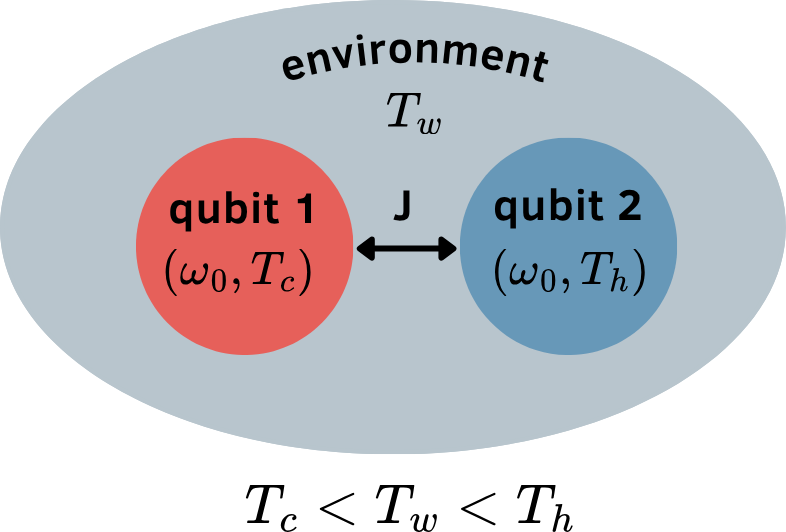
\includegraphics[width=0.35\linewidth]{Images/Qubits/model-2-qubits.png}
    \caption{Model for two interacting qubits with a global bath.}
    \label{fig:model-2-qubits}
\end{figure}

We focus on only two qubits ($N=0$) coupled to a global bath as shown in Fig. 1. Both qubits have an energy gap of $h = \frac{\omega_0}{2}$ with one of them heating up from the temperature $T_c$ while the other is cooling down from the temperature $T_h$, and the bath is at an intermediate temperature $T_w$. To genuinely heat up or cool down the qubits, they must be thermal states, allowing the definition of a physical temperature. If we added off-diagonal elements to a qubit's density matrix, it would only be possible to define an effective temperature, making the terms ``heating” and ``cooling” inaccurate. Therefore, we introduce initial global coherences while keeping the reduced state of each qubit thermal throughout the dynamics, resulting in the density matrix
\begin{equation}
    \rho = \rho_{c} \otimes \rho_{h} + \chi,
\end{equation}

\noindent where $\rho_c$ and $\rho_h$ are the thermal states of the cold and hot qubits, respectively, and the global coherences are given by $\chi = e \ket{01}\bra{10} + e^* \ket{10}\bra{01} + f \ket{00}\bra{11} + f^* \ket{11}\bra{00}$ in the computational basis and has $\text{Tr}_c[\chi] = \text{Tr}_h[\chi] = 0$. The density matrix is always positive semi-definite, imposing constraints on the values of the coherence parameters $|e|$ and $|f|$. By diagonalizing $\rho$, we obtain that the maximum value for $|e|$ and $|f|$ is $1/\mathcal{Z}_c \mathcal{Z}_h$, with $\mathcal{Z}$ being the partition function. The detailed calculation can be found in \textcolor{red}{apx:max-coherence}.

The last step before discussing our results is to define $T_c$ and $T_h$. To make a fair comparison between heating and cooling, we must find thermodynamically equidistant initial states from equilibrium. Given that the asymmetry only appears for far-from-equilibrium systems, we quantify this distance using the nonequilibrium free energy ($F_{neq}$ defined by \textcolor{red}{Eq.}) \cite{krissia-2024}. Additionally, because $F_{neq}$ is directly related to the relative entropy (defined by \textcolor{red}{Eq.}), initial states that are thermodynamically equidistant from equilibrium also have the same relative entropy from the steady state of the dynamics. In our case, we compare the cold and hot qubits' initial states with their local steady state ($\rho_{ss}^q$),
\begin{equation}
    D[\rho_c || \rho_{ss}^{q}] = D[\rho_h || \rho_{ss}^{q}].
    \label{eq:same-D-qubit}
\end{equation}

\noindent By definition, a steady state does not change with time, which can be found by solving $\mathcal{L}( \rho_{ss}^G) = 0$, where $\rho_{ss}^G$ is the global steady state, and $\mathcal{L}$ is the generator of the dynamics as discussed in Chap. \ref{cap:oqs}. However, from Sec. \ref{sec:davies-maps}, we know that the steady state of a Davies map is always a Gibbs state, 
\begin{equation}
    \rho_{ss}^G = \frac{e^{-\beta_w H_S}}{\mathcal{Z}_S},
\end{equation} 

\noindent where $\beta_w = 1/T_w$, $H_S$ is the system Hamiltonian (Eq. \eqref{eq:HS-qubit}) and $\mathcal{Z}_S$ is the partition function. Then, we can trace out one of the qubits to find $\rho_{ss}^q$. Because in a global bath both qubits equilibrate to the same temperature, it makes no difference which one we trace out. However, it should be emphasised that, even though the global system thermalises to the bath's temperature, the qubit's temperature of equilibrium is different. This happens because the interaction between the qubits generates correlations that are erased by the partial trace.

Now that we discussed the interaction model between the qubits and the structure of the initial state, we can solve the master equation given by the Davies maps presented in Chap. \ref{cap:oqs}. With the local density matrices, we compute the Quantum Fisher Information defined in \textcolor{red}{Eq.}. Then, we obtain the thermal kinematics variables presented in \textcolor{red}{Chapter 3} to analyse the thermal relaxation asymmetry of our system.

%%%%%%%%%%%%%%%%%%%%%%%%%%%%%%%%%%%%%%%%%%%%%%%%%%%
\subsection{Results for the XX Model}\label{sec:result-xx}

This section presents the results regarding the heating and cooling asymmetry for the XX model ($\gamma = 0$ and $\Delta = 0$). From the Hamiltonian in Eq. \eqref{eq:HS-qubit}, used $h = \omega_0 / 2$ and redefined $g = 2J$. For this model, the qubit local steady state is

\begin{equation}
    \rho_{ss}^q = \frac{1}{\mathcal{Z}_q}
    \begin{bmatrix}
        e^{\beta_w \omega_0} + \cosh (\beta_w J) & 0\\
        0 & e^{-\beta_w \omega_0} + \cosh (\beta_w J)
    \end{bmatrix},
\end{equation}

\noindent where $\mathcal{Z}_q = 2 \cosh(\beta_f \omega_0) + 2 \cosh(\beta_f J)$. The local temperature of this state is
\begin{equation}
    \beta_{qubit}^{f} = \frac{1}{\omega_0} \ln \left( \frac{e^{\beta_w \omega_0} + \cosh (\beta_w J)}{e^{-\beta_w \omega_0} + \cosh (\beta_w J)} \right),
\end{equation}

\noindent that is different from the bath's temperature. Using this result, the initial temperatures $T_c$ and $T_h$ are obtained numerically from Eq. \eqref{eq:same-D-qubit}, ensuring a fair comparison between heating and cooling.

With these temperatures defined, we can compare the dynamics of the heating and cooling qubits. In our results, heating and cooling are represented in red and blue, respectively. Dashed lines indicate the non-interaction case ($J = 0$), while solid lines represent the interaction case ($J = 0.8$). The degree of completion (\textcolor{red}{Eq.}) is shown in Fig. \ref{fig:completion-xx} for the case without initial coherence (left) and the case with maximum initial coherence (right). Given that the red lines are always above their corresponding blue lines, we conclude that heating is faster than cooling. Using this same idea, we see that the interaction between qubits allows a faster relaxation. Furthermore, only for the interaction case, the initial coherence seems to affect the intermediary dynamics by delaying cooling, which increases the asymmetry while keeping the total relaxation time unchanged. These same observations can be obtained from the statistical velocity (\textcolor{red}{Eq.}) shown in Fig. \ref{fig:velocity-xx}.

\begin{figure}[t]
    \centering
    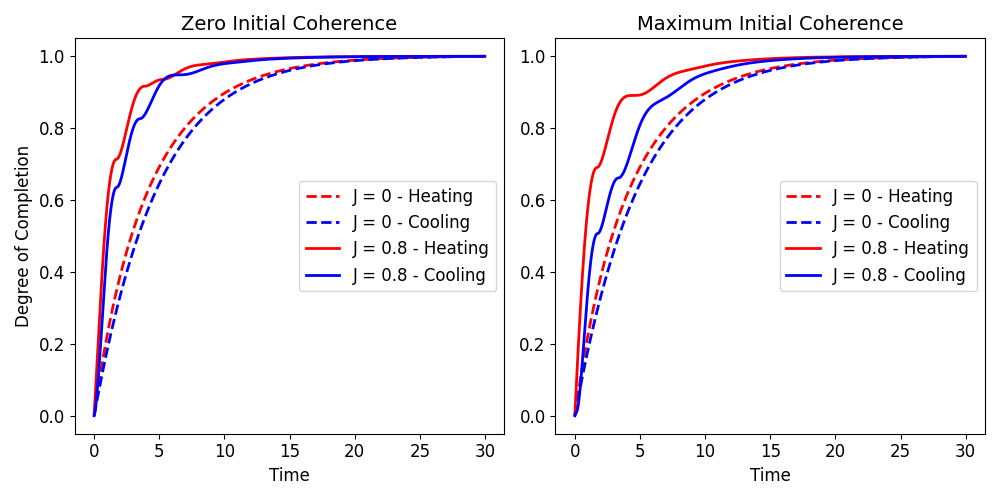
\includegraphics[width=0.8\linewidth]{Images/Qubits/XX/completion-xx.png}
    \caption{Degree of completion for XX-model. Each line correspond to cooling (blue) or heating (red) processes with (solid) or without (dashed) interaction between qubits.}
    \label{fig:completion-xx}
\end{figure}

\begin{figure}[t]
    \centering
    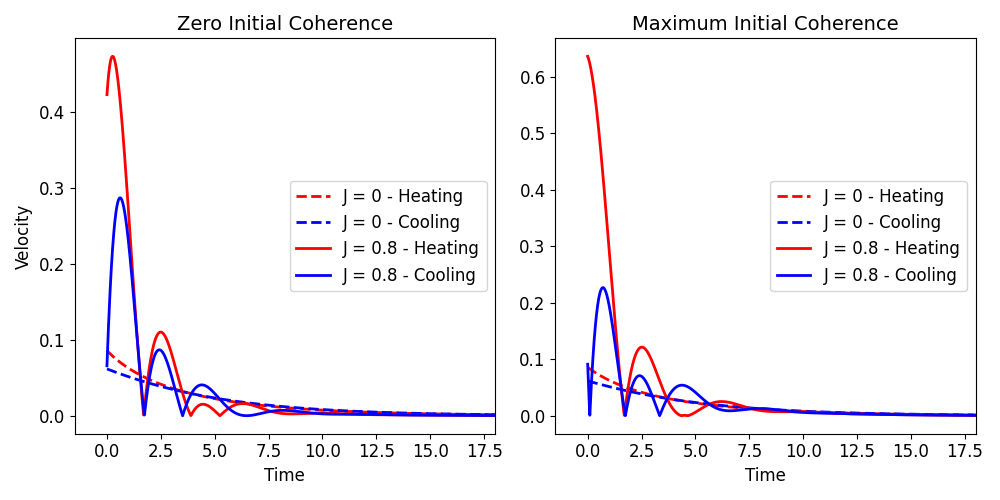
\includegraphics[width=0.8\linewidth]{Images/Qubits/XX/velocity-xx.png}
    \caption{Statistical velocity for XX-model. Each line correspond to cooling (blue) or heating (red) processes with (solid) or without (dashed) interaction between qubits.}
    \label{fig:velocity-xx}
\end{figure}

In addition to our previous observations, note that both the statistical velocity and the degree of completion have oscillations. To understand better its cause, we calculated the entropy production rate ($\Pi_\rho$ defined by \textcolor{red}{Eq.}) that is shown in Fig. \ref{fig:sprod-xx}. Only for the interaction case, the entropy production rate becomes negative for some time intervals, which is a witness of non-Markovian dynamics, where information from the environment returns to the systems \cite{popovic-2018}. Another interesting observation is that heating has a bigger initial entropy production rate than cooling, which corroborates with the hypothesis that heating is faster because its entropy increases faster than cooling decreases its energy \cite{ibanez-2024}.

\begin{figure}[t]
    \centering
    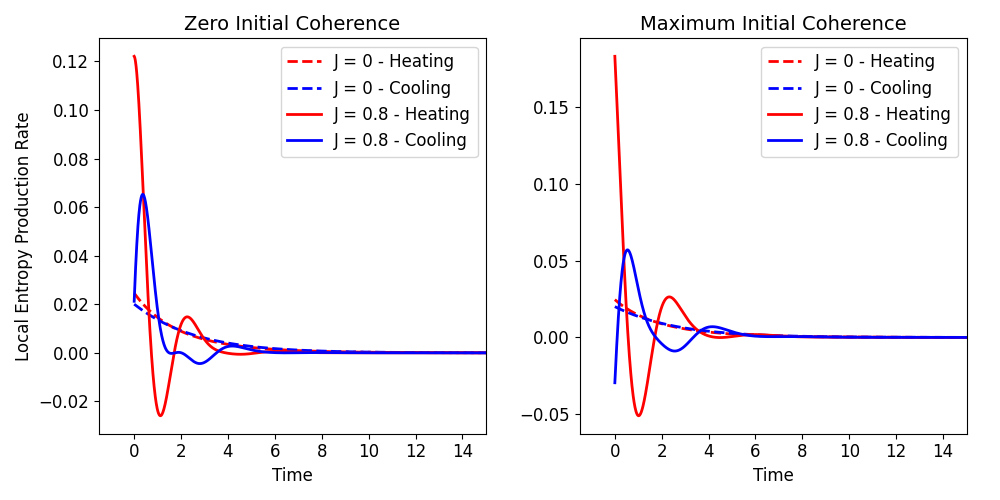
\includegraphics[width=0.8\linewidth]{Images/Qubits/XX/sprod-xx.png}
    \caption{Entropy production rate for the XX-model. Each line corresponds to cooling (blue) or heating (red) processes with (solid) or without (dashed) interaction between qubits.}
    \label{fig:sprod-xx}
\end{figure}

\begin{figure}[b!]
    \centering
    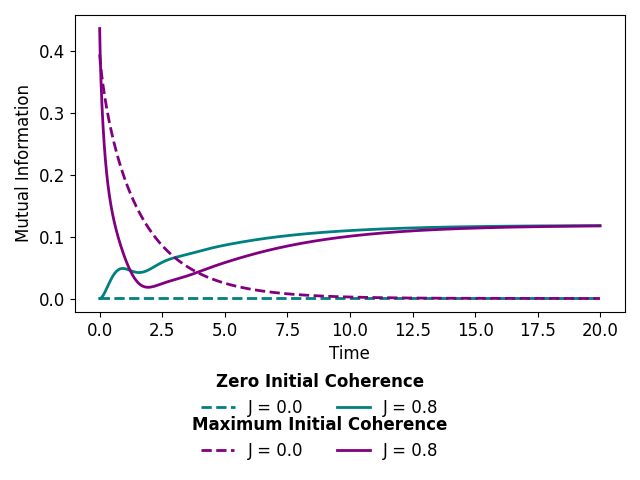
\includegraphics[width=0.5\linewidth]{Images/Qubits/XX/MI-xx.png}
    \caption{Mutual information as a function of time for the zero (teal) and maximum (purple) initial coherence with $J=0$ (dashed) and $J=0.8$ (solid) cases.}
    \label{fig:mi-xx}
\end{figure}

\begin{figure}[b!]
    \centering
    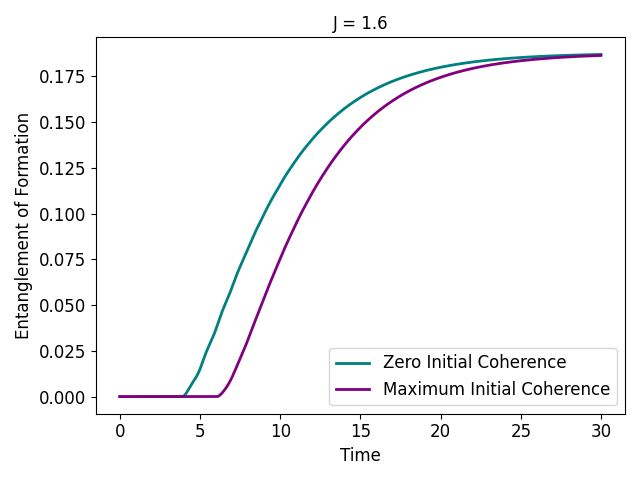
\includegraphics[width=0.5\linewidth]{Images/Qubits/XX/EoF-xx.png}
    \caption{Entanglement of formation as a function of time for the zero (teal) and maximum (purple) initial coherence with $J=1.6$.}
    \label{fig:eof-xx}
\end{figure}

Another interesting behaviour of the interaction case is that it generates correlations that are signalised by the mutual information defined in \textcolor{red}{Eq.}. Until this moment, we used an interaction that do not create entanglement between the qubits despite of generating correlations as shown in Fig. \ref{fig:mi-xx}. Now, let's compare what happens to the asymmetry when we have the entanglement formation. For $J=1.6$ we see in Fig. \ref{fig:eof-xx} that the entanglement of formation (\textcolor{red}{Eq.}) increases with time until reaching a plateau in the equilibrium. It is interesting that the presence of maximum initial coherence delays the generation of entanglement. In Fig. \ref{fig:completion-all-J-xx} we see that the presence of entanglement (solid lines) makes the thermal relaxation more symmetric and slower when compared to the $J=0.8$ case (dashed lines), but still is faster than the non-interacting case. Again the initial coherence do not change the overall thermalisation, but affects the beginning of the dynamics by making a small increase of the asymmetry.

\begin{figure}[t]
    \centering
    
\includegraphics[width=0.9\linewidth]{Images/Qubits/XX/completion-assimetria-xx.png}
    \caption{Degree of completion for heating (red) and cooling (blue) states with zero (left) or maximum (right) initial coherence. The interaction parameters used are $J=0$ (dotted), $J=0.8$ (dashed), and $J=1.6$ (solid).}
    \label{fig:completion-all-J-xx}
\end{figure}


%%%%%%

\section{Gaussian States}\label{sec:gaussian}

% Quantisized fields and canonical operators 
% Phase-space, characteristic functions and quasi-probabilities distributions
% Gaussian states: mean vector and covariance matrix
% Gaussian operators: displacement and squeezing
% Ergotropy
% Wigner relative entropy
% Wigner entropy
 


Continuous-variable (CV) systems are described by observables with continuous spectra, typically associated with infinite-dimensional Hilbert spaces. An important example is the quantised electromagnetic field, whose modes behave as independent harmonic oscillators. Despite being described by continuous variables, the energy of each mode is quantised in equally spaced levels, with transitions occurring through the absorption or emission of energy quanta known as photons. For simplicity, let us consider an electromagnetic field inside an optical cavity, where only $N$ relevant modes are taken into account. In this case, the Hamiltonian can be written as the sum of independent modes, $H = \sum_{k=1}^{N} H_k$, with each mode described by the harmonic oscillator Hamiltonian,
\begin{equation}
    H_k = \hbar \omega_k \left( \hat{a}_k^\dagger \hat{a}_k + \frac{1}{2} \right).
    \label{eq:k-harmonic-oscillator}
\end{equation}

\noindent Here, $\hat{a}_k^\dagger$ and $\hat{a}_k$ are the creation and annihilation operators of the mode $k$. The origin of these names is that they create or annihilate a photon with wave vector $\mathbf{k}$, changing the mode energy by one quantum. $\hat{a}_k^\dagger$ and $\hat{a}_k$ satisfy the following commutation relations
\begin{align}
    &[\hat{a}_i, \hat{a}_j^\dagger] = \delta_{ij},\\
    &[\hat{a}_i^\dagger, \hat{a}_j^\dagger] = [\hat{a}_i, \hat{a}_j] = 0.
\end{align}

\noindent The quantum harmonic oscillator can equivalently be described in terms of the position and momentum operators, also called quadratures,
\begin{align}
    &\hat{q}_k = \frac{1}{\sqrt{2}} (\hat{a}_k^\dagger + \hat{a}_k)\\
    &\hat{p}_k = \frac{i}{\sqrt{2}} (\hat{a}_k^\dagger - \hat{a}_k).
\end{align}

\noindent For an $N$-mode systems, the quadratures can be grouped into a vector $\hat{R} = (\hat{R}_1, \dots, \hat{R}_N)^T = (\hat{q}_1, \hat{p}_1, ..., \hat{q}_N, \hat{p}_N)^T$, allowing the commutation relations to be condensed in $[\hat{R}_i, \hat{R}_j] = i \Omega_{ij}$, where
\begin{equation}
    \Omega = \bigoplus_{k = 1}^{N}
    \begin{bmatrix}
        0 & 1\\
        -1 & 0
    \end{bmatrix}.
\end{equation}

\noindent is the $N$-mode symplectic form. The quadratures operators define the phase space $\mathcal{P} = (\mathbb{R}^{2N} , \Omega)$, a real 2N-dimensional space provided with the symplectic structure $\Omega$. This structure encodes the Heisenberg uncertainty principle. As a consequence, quantum states are represented as phase-space regions instead of single points like in classical mechanics.

The eigenstates of each Hamiltonian $H_k$ in Eq. \eqref{eq:k-harmonic-oscillator} are the Fock states $\ket{n}_k$, where $n$ denotes the number of photons in mode $k$. As a consequence, the basis for the full multimode Hamiltonian is given by the tensor product $\ket{n}_\mathbf{k} = \ket{n}_1 \otimes \ket{n}_2 \otimes \dots \otimes \ket{n}_N$. Each Fock basis is bounded from below by the vacuum state $\ket{0}_k$, defined by $\hat{a}_k \ket{0}_k = 0$. Although the Fock representation is important for describing quantised fields, it becomes less convenient when dealing with states containing a large number of photons, such as laser fields. In these cases, an alternative representation is to use coherent states. A single-mode coherent state can be written as a linear combination of Fock states,
\begin{equation}
    \ket{\alpha}_k = e^{-\frac{1}{2}|\alpha|^2} \sum_{n=0}^{\infty} \frac{\alpha^n}{\sqrt{n!}} \ket{n}_k.
\end{equation}

\noindent Experimentally, coherent states may be generated by applying the Weyl operator, also known as the displacement operator, to the vacuum state,
\begin{equation}
    \ket{\alpha}_k = \hat{D}_k (\alpha) \ket{0}_k,
\end{equation}

\noindent where the Weyl operator is
\begin{equation}
    \hat{D}_k (\alpha) = e^{\alpha \hat{a}_k^\dagger - \alpha^* \hat{a}_k},
    \label{eq:displacement-single-mode}
\end{equation}

\noindent with $\alpha \in \mathbb{C}$ being the displacement parameter. For the $N$-mode case, the displacement operator can be written in terms of the canonical operator vector $\hat{R}$ as
\begin{equation}
    \hat{D}(\mathbf{r}) = e^{\hat{R}^T \Omega \mathbf{r}},
\end{equation}

\noindent where $\mathbf{r} = (q_1', p_1', \dots, q_N', p_N')$ is a vector in phase-space $\mathcal{P}$ specifying the displacement applied for each quadrature.

Until this moment, we have been using density matrices to describe our states. However, the density operators of CV systems are infinite-dimensional, making this approach mathematically complicated. An alternative is to work with equivalent phase-space representations. The characteristic function is a multivariable function obtained through the Fourier-Weyl transform of the density operator \cite{serafini-book}, being written as
\begin{equation}
    \chi_\rho (\mathbf{r}) = \text{Tr} [\rho \hat{D}(\mathbf{r})].
\end{equation}

\noindent In this work, we will consider only the symmetric-ordered characteristic function defined above; other orderings can be found in Refs. \cite{gerardo-2014, serafini-book}. Although $\chi_\rho$ fully characterises a quantum state, it is still expressed in terms of displacement variables rather than quadrature operators. The full transition to phase-space can be done by taking the Fourier transform of the characteristic function, resulting in the Wigner quasiprobability distribution,
\begin{equation}
    W_\rho (\mathbf{q}, \mathbf{p}) = \frac{1}{\pi^N} \int_{\mathbb{R}^{N}} \bra{\mathbf{q} + \mathbf{q'}} \rho \ket{\mathbf{q} - \mathbf{q'}} e^{2i \mathbf{q'.p}} d^N \mathbf{q'}.
\end{equation}

\noindent The derivation of the Wigner distribution is in \textcolor{red}{apx:wigner}. Here, $\mathbf{q}$ and $\mathbf{p}$ are $N$-dimensional vectors indicating the coordinates of a point in the phase-space. The vector $\mathbf{x}$ is a symmetric displacement around $\mathbf{q}$, being the integration variable and $\hat{q}_k \mathbf{x} = q_k \mathbf{x}$. The Wigner distribution is called a quasiprobability because, unlike classical probability distributions, it may take negative values. Still, its marginalisation reproduces the correct probability distribution associated with the quadrature observables \cite{gerardo-2014}.

Among the different classes of continuous-variable states, Gaussian states play an important role due to their mathematical simplicity and experimental relevance. As the name suggests, the Wigner distribution associated with these states is a Gaussian function in phase space. For a single variable, a Gaussian function can be written as
\begin{equation}
    g(x) = \frac{1}{\sqrt{2\pi} \sigma} \exp \left(-\frac{1}{2} \frac{(x - \mu)^2}{\sigma^2} \right),
\end{equation}

\noindent where $\mu = \braket{x}$ is the mean value (first moment) and $\sigma^2 = \braket{(x -  \braket{x})^2}$ is the variance (second moment). These two quantities fully characterise a Gaussian distribution. Similarly, multimode Gaussian states are fully characterised by the first and second moments of the quadrature operators. The first moments are grouped into the mean vector $\mathbf{v}$, whose elements are
\begin{equation}
    v_j = \braket{\hat{R}_j}_\rho,
\end{equation}

\noindent while the second moments are written in the covariance matrix $\Theta$, with elements
\begin{equation}
    \Theta_{ij} = \frac{1}{2}\braket{\hat{R}_i \hat{R}_j + \hat{R}_j \hat{R}_i}_\rho - \braket{\hat{R}_i}_\rho \braket{\hat{R}_j}_\rho,
\end{equation}

\noindent where $\braket{\hat{O}}_\rho \equiv \text{Tr}[\rho \hat{O}]$. With these definitions, the Wigner distribution becomes
\begin{equation}
    W_\rho (\mathbf{x}) = \frac{1}{\pi^N \sqrt{|\Theta|}} \exp \left( -(\mathbf{x} - \mathbf{v})^T \Theta^{-1} (\mathbf{x} - \mathbf{v}) \right),
\end{equation}

\noindent where $\mathbf{x} \in \mathbb{R}^{2N}$ and $|\Theta| = \det(\Theta)$. Important examples of Gaussian states are coherent states, thermal states, and the vacuum state.

In addition to characterising Gaussian states, we are interested in the operations that act upon them. Although general quantum operations may destroy Gaussianity, Gaussian operations preserve the Gaussian form of the state in phase space. In this work, we focus specifically on displacement operations, defined in Eq. \eqref{eq:displacement-single-mode}, and squeezing operations.

The displacement operator, as the name suggests, shifts the whole Gaussian state without deforming the distribution. In other terms, it varies the mean vector while keeping the covariance matrix unchanged. On the other hand, the squeezing operator for a single mode is defined as
\begin{equation}
    \hat{S}_k (z) = e^{-\frac{1}{2} (z^* \hat{a}_k - z \hat{a}_k^\dagger)},
\end{equation}

\noindent where $z = r e^{i\phi_s}$ with $r$ being the squeezing parameter and $\phi_s$ being the squeezing phase responsible to rotate the state. The squeezing operator deforms the state in the phase space by compressing one quadrature. As a consequence of the uncertainty principle, the other quadrature will expand. Mathematically, this means that squeezing operations only affect the covariance matrix, preserving the mean vector. An illustration of how these operations affect a Gaussian state is shown in Figure \ref{fig:gaussian-operations}. We will not use the multimode squeezing operator in this work, but its definitions can be found in Refs. \cite{gerardo-2014, serafini-book}.

\begin{figure}[t]
    \centering
    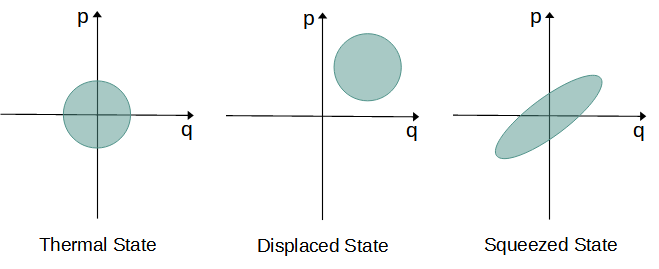
\includegraphics[width=0.6\linewidth]{Images/Gaussian/gaussian-operations.png}
    \caption{Illustration of a single-mode thermal state, displaced coherent state, and squeezed coherent state in the phase space.}
    \label{fig:gaussian-operations}
\end{figure}

From a thermodynamic perspective, squeezing and displacement operations add energy to the system, bringing it to the far-from-equilibrium regime \cite{huber-2016}. One way to quantify this energy gain is by a quantity called ergotropy, which is defined as the maximum amount of energy that can be extracted from a state via cyclic unitary operations \cite{medina-2025},
\begin{equation}
    \mathcal{E}(\hat{\rho}, \hat{H}) = E(\hat{\rho}) - E(\hat{\pi}),
\end{equation}

\noindent where $E(\hat{\rho}) = \text{Tr}[\hat{\rho} \hat{H}]$ is total energy of the system and $E(\hat{\pi}) = \min_{\hat{U}} \text{Tr}[\hat{U} \hat{\rho} \hat{U}^\dagger \hat{H}]$ is the energy of the correspondent state that no work can be extracted via unitary operations, being called \textit{passive state} and represented by $\hat{\pi}$. For Gaussian states, all passive states are thermal. That said, the ergotropy for a Gaussian state $W$ with mean vector $\mathbf{v}$ and covariance matrix $\Theta$ is defined as
\begin{equation}
    \mathcal{E}(W) = \omega f(\beta_\pi) K[W || W_\pi],
\end{equation}

\noindent where $W_\pi$ is the Wigner function of the passive state, $f(\beta_\pi) = \sqrt{|\Theta|}$ being $\beta_\pi$ the inverse temperature of the passive state, and $K$ is the Wigner relative entropy defined as
\begin{equation}
   K[W_1 || W_2] = -1 + \frac{1}{2} \left[(\mathbf{v}_1 - \mathbf{v}_2)^\dagger \Theta_2^{-1} (\mathbf{v}_1 - \mathbf{v}_2) + \text{Tr}(\Theta_2^{-1} \Theta_1) + \ln \frac{|\Theta_2|}{|\Theta_1|} \right].
   \label{eq:wigner-relative-entropy}
\end{equation}

Recently, it was shown in Ref. \cite{medina-2025} that the relaxation of squeezed states is faster than that of a displaced state with the same initial ergotropy. These results inspired the study of how displacement and squeezing may affect the thermal relaxation asymmetry. In Section \ref{sec:result-gaussian}, we will see how Gaussian states evolve in time and will redefine the thermal kinematics variables for them.


\subsection{Thermal Relaxation of Gaussian States}\label{sec:result-gaussian}

% Evolução: equação de lyapunov
% Wigner-Fisher information
As discussed in Chap. \ref{cap:oqs}, the dynamics of an open system can be described by the Lindblad master equation. In our case, we will consider a single bosonic mode (Eq. \eqref{eq:k-harmonic-oscillator} with $k=1$) interacting with a thermal bath, which has already been derived in Sec. \ref{sec:example},
\begin{equation}
    \frac{d}{dt} \hat{\rho} = -i [\hat{H}, \hat{\rho}] + \Gamma (\bar{n}+1) \mathcal{D}_\alpha(\hat{\rho}) + \Gamma \bar{n}\mathcal{D}_{\alpha^\dagger} (\hat{\rho}),
    \label{eq:lindblad-gaussian}
\end{equation}

\noindent where $\Gamma$ is the dissipation rate, $\bar{n} = 1/(e^{\beta \omega} - 1)$ is the Bose distribution, and $\mathcal{D}_L (\hat{\rho}) = L \hat{\rho} L^\dagger - \frac{1}{2}\{L^\dagger L, \hat{\rho} \}$ is the dissipator. As elaborated in the previous section, it is convenient to use the phase-space representation instead of the density matrix. For this reason, we use Eq. \eqref{eq:lindblad-gaussian} in $\frac{d}{dt} \braket{A}_\rho = \text{Tr}[A \frac{d}{dt}\rho]$ to find the differential equations for the mean vector and covariance matrix.

The mean vector of a single mode has the form $\mathbf{v}_t = (\braket{\hat{a}}, \braket{\hat{a}^\dagger})^T$. To find its time derivative, we compute
\begin{align}
    &\frac{d}{dt}\braket{\hat{a}} = -\left( i\omega + \frac{\Gamma}{2} \right) \braket{\hat{a}}\\
    &\frac{d}{dt}\braket{\hat{a}^\dagger} = \left( i\omega - \frac{\Gamma}{2} \right) \braket{\hat{a}^\dagger},
\end{align}

\noindent which gives the differential equation 
\begin{equation}
    \dot{\mathbf{v}}_t = \Lambda \mathbf{v}_t,
    \label{eq:dt-mean-vector}
\end{equation}
\noindent where
\begin{equation}
    \Lambda = -\frac{1}{2}
    \begin{bmatrix}
        \Gamma + 2i\omega & 0\\
        0 & \Gamma - 2i\omega
    \end{bmatrix}.
\end{equation}

\noindent The covariance matrix of a single mode is structured as
\begin{equation}
    \Theta_t =
    \begin{bmatrix}
        \frac{1}{2}(\braket{\hat{a}^\dagger \hat{a}} + \braket{\hat{a} \hat{a}^\dagger}) - \braket{\hat{a}^\dagger} \braket{\hat{a}} & \braket{\hat{a}^2} - \braket{\hat{a}}^2\\
        \braket{\hat{a}^{\dagger 2}} - \braket{\hat{a}^\dagger}^2 & \frac{1}{2}(\braket{\hat{a}^\dagger \hat{a}} + \braket{\hat{a} \hat{a}^\dagger}) - \braket{\hat{a}^\dagger} \braket{\hat{a}}
    \end{bmatrix}.
\end{equation}

\noindent To take its time derivative, we first compute
\begin{align}
    &\frac{d}{dt}\braket{\hat{a} \hat{a}^\dagger} = -\Gamma (\braket{\hat{a}\hat{a}^\dagger} - \bar{n} - 1),\\
    &\frac{d}{dt}\braket{\hat{a}^\dagger \hat{a}} = -\Gamma (\braket{\hat{a}\hat{a}^\dagger} - \bar{n}),\\
    &\frac{d}{dt}\braket{\hat{a}^2} = -(2i\omega + \Gamma)\braket{\hat{a}^2},\\
    &\frac{d}{dt}\braket{\hat{a}^{\dagger 2}} = (2i\omega - \Gamma)\braket{\hat{a}^{\dagger 2}},
\end{align}

\noindent to obtain the following differential equation called the Lyapunov Equation,
\begin{equation}
    \dot{\Theta}_t = \Lambda \Theta + \Theta \Lambda^\dagger + F,
    \label{eq:lyapunov}
\end{equation}

\noindent where $F = \Gamma f(\beta) \mathbb{I}$. Therefore, by solving Eqs. \eqref{eq:dt-mean-vector} and \eqref{eq:lyapunov}, we find that the time evolution of a single-mode Gaussian state is given by
\begin{align}
    &\mathbf{v}_t = e^{-\Gamma t} (\braket{a}_0 e^{-i \omega t}, \braket{a^\dagger}_0 e^{i \omega t})^T\\
    &\Theta_t^{11} = \Theta_t^{22} = c_{0} e^{-\Gamma t} + f(\beta),\\
    &\Theta_t^{12} = (\Theta_t^{21})^* = d_{0} e^{-(\Gamma + 2i\omega)t},
\end{align}

\noindent where $c_0$, $d_0$, $\braket{a}_0$, and $\braket{a^\dagger}_0$ are constants obtained from the initial conditions.

After finding the dynamics of a single-mode Gaussian state, we are now ready to investigate the heating and cooling asymmetry in these systems. As discussed in \textcolor{red}{Chapter 3}, Fisher Information is the essential quantity for the thermal kinematics approach of thermal relaxation asymmetry. For single-mode Gaussian systems, we can find the Wigner-Fisher Information by making a Taylor expansion of $K[W_{t+dt} || W_t]$ (the derivation is in \textcolor{red}{apx:wigner-fisher}), resulting in
\begin{equation}
    \mathcal{I}_W (t) = \dot{\vec{v}}_t^\dagger \Theta^{-1}_t \dot{\vec{v}}_t + \text{Tr}[(\Theta_t^{-1} \dot{\Theta}_t)^2],
    \label{eq:wigner-fisher}
\end{equation}

Having introduced the necessary formalism, we will start discussing our results. Although the heating and cooling asymmetry for Gaussian thermal states has already been calculated with numerical methods \cite{tejero-2025}, the following section presents an analytical treatment of this problem.

\subsubsection{Asymmetry for Thermal States}\label{sec:result-thermal}

In this section, we consider a Gaussian state initially in a thermal state with inverse temperature $\beta_i$ interacting with a bath at inverse temperature $\beta_f$. The system's dynamics is described by a zero mean vector ($\mathbf{v}_t = 0$) and a covariance matrix equal to $\Theta_t = \Delta_\beta \mathbb{I}$, being $\Delta_{\beta} = [f(\beta_i) - f(\beta_f)]e^{-\Gamma t} + f(\beta_f)$ where $\Gamma$ is the dissipation rate, $t$ is the time and $f(\beta) = \bar{n} + 1/2$.

Similar to the qubits case, to find two thermodynamically equivalent initial states, we use the Wigner relative entropy defined in Eq. \eqref{eq:wigner-relative-entropy}. For thermal states, $|\Theta| = (\Delta_\beta)^2$ and $\Theta^{-1} = \frac{1}{\Delta_\beta} \mathbb{I}$, being $\lim_{t\rightarrow\infty} \Delta_\beta = f(\beta_f)$ in equilibrium. Using this, we obtain that the Wigner relative entropy for a thermal state is
\begin{equation}
    K[W_t || W_f] = -1 + \frac{\Delta_\beta}{f(\beta_f)} + \ln \frac{f(\beta_f)}{\Delta_\beta}.
    \label{eq:K-thermal}
\end{equation}

\noindent The analytical expression for the Wigner-Fisher Information (defined in Eq. \eqref{eq:wigner-fisher}) is
\begin{equation}
    \mathcal{I}_{W} (t) = 2 \left[ \frac{\partial}{\partial t} \ln \Delta_\beta \right]^2,
\end{equation}

\noindent the statistical velocity (defined in \textcolor{red}{Eq.})
\begin{equation}
    v_{W}(t) = \frac{\partial}{\partial t} \ln \Delta_\beta,
\end{equation}

\noindent and the statistical length (defined in \textcolor{red}{Eq.})
\begin{equation}
     \mathcal{L}_{W} (t) = \ln \left( \frac{[f(\beta_i) - f(\beta_f)]e^{-\Gamma t} + f(\beta_f)}{f(\beta_i)} \right).
     \label{eq:L-termico}
\end{equation}

\noindent Note that the statistical length in equilibrium is

\begin{equation}
    \mathcal{L}_{W}^{eq} \equiv \lim_{t \rightarrow \infty} \mathcal{L}_W (t) = \ln\left[ \frac{f(\beta_f)}{f(\beta_i)} \right],
    \label{eq:L-termico-eq}
\end{equation}

\noindent which means that, if there are two states with different initial temperatures that relaxate to the same final temperature, their statistical length will be different. Lets define $f_i \equiv f(\beta_f)/f(\beta_i)$ and $k = \exp(-\Gamma t)$, and use the expressions \eqref{eq:L-termico} and \eqref{eq:L-termico-eq} to write the degree of completion as
\begin{equation}
    \varphi(k) = \frac{\ln (k + (1-k)f_i)}{\ln(f_i)}.
\end{equation}

Now, we can analyse the thermal relaxation asymmetry for thermal states. First, we can use the Jensen inequality for $f(x) = \ln(x)$ to find that
\begin{equation}
    \ln(k + (1 - k) f_i) \geq (1-k) \ln(f_i).
\end{equation}

\noindent We know that $\beta_c > \beta_f > \beta_h$, which results in $f(\beta_c) < f(\beta_f) < f(\beta_h)$, leading to 
\begin{align}
    &1 > \frac{f(\beta_f)}{f(\beta_h)} = f_h \label{ineq:fbeta-cooling}\\
    &1 < \frac{f(\beta_f)}{f(\beta_c)} = f_c. \label{ineq:fbeta-heating}
\end{align}

\noindent This means that $\ln(f_c) > 0$ and the heating degree of completion ($\varphi_c$) is
\begin{equation}
    \varphi_c = \frac{\ln (k + (1-k)f_c)}{\ln(f_c)} \geq 1-k.
\end{equation}

\noindent On the other hand, $\ln(f_h) < 0$ and the cooling degree of completion ($\varphi_h$) is
\begin{equation}
    \varphi_h = \frac{\ln (k + (1-k)f_h)}{\ln(f_h)} \leq 1-k.
\end{equation}

\noindent With this, we conclude that heating is always faster than cooling for Gaussian thermal states ($\varphi_c \geq \varphi_h$).

It is relevant to study whether the presence of thermal relaxation asymmetry in Gaussian systems is also explained by the difference in entropy production rate. Taking the negative of the time derivative of Wigner relative entropy (Eq. \eqref{eq:K-thermal}), we find that the entropy production rate is
\begin{equation}
    \Pi_W = \frac{\dot{\Delta}_\beta}{\Delta_\beta} - \frac{\dot{\Delta}_\beta}{f(\beta_f)}.
\end{equation}

\begin{figure}[b!]
    \centering
    
\includegraphics[width=0.6\linewidth]{Images/Gaussian/Sprod-thermal.png}
    \caption{Entropy production rate for heating (red) and cooling (blue) thermal states.}
    \label{fig:sprod-thermal}
\end{figure}

\noindent From this expression, we obtain Fig. \ref{fig:sprod-thermal} by using $K[W_c || W_f] = K[W_h || W_f] = 0.5$ and $T_f = 2$ (in natural units). Note that heating reaches zero before cooling, corroborating our conclusion that heating relaxes faster than cooling. Also, heating has an initially higher entropy production rate than cooling, which explains the asymmetry.


\subsubsection{Asymmetry for Displaced States}\label{sec:result-displaced}

After displacing a thermal state, the mean vector becomes $\vec{v}_t = (\mu_t, \mu_t^*)$ where $\mu_t = \mu e^{-(i\omega + \Gamma / 2)t}$ while the covariance matrix remains unchanged, i.e., $\Theta_t = \Delta_\beta \mathbb{I}$. Using these results in the Wigner relative entropy (Eq. \eqref{eq:wigner-relative-entropy}), we find
\begin{equation}
    K[W_t || W_f] = -1 + \frac{|\mu|^2}{f(\beta_f)} e^{-\Gamma t} + \frac{\Delta_\beta}{f(\beta_f)} + \ln \frac{f(\beta_f)}{\Delta_\beta}.
\end{equation}

\noindent Term containing the displacement parameter ($\mu$) is independent of the system's initial temperature, which means that, regardless of the initial temperature, applying a displacement operator to any thermal state results in the same shift in their Wigner relative entropy. Thus, for simplicity, we chose two equidistant thermal states and then applied the same amount of work on both (which is equivalent to using the same $\mu$). As we did before, we could try to analytically calculate the thermal kinematics variables, but the Wigner-Fisher Information for a displaced state is
\begin{equation}
    I_W (t) = \frac{2}{\Delta_\beta} \left[ \frac{\dot{\Delta}_\beta^2}{\Delta_\beta} + \left(\omega^2 + \frac{\Gamma^2}{4} \right)|\mu|^2 e^{-\Gamma t} \right],
\end{equation}

\begin{figure}[b!]
    \centering
    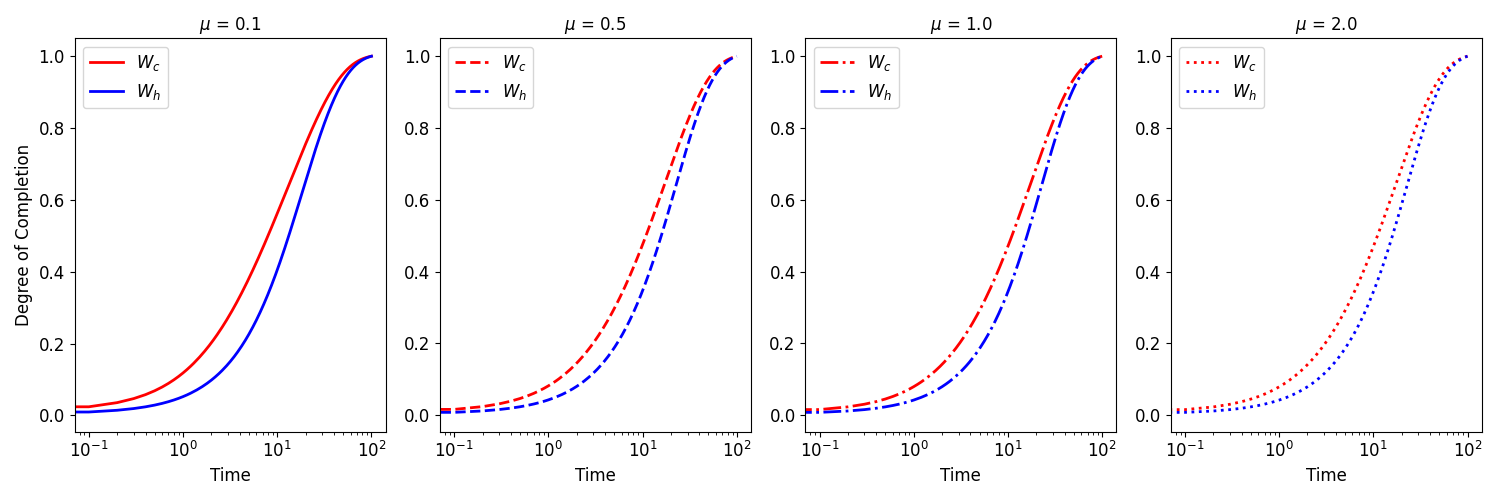
\includegraphics[width=\linewidth]{Images/Gaussian/completion-displaced.png}
    \caption{Degree of completion for a displaced thermal state. Each graph corresponds to a different displacement parameter ($\mu$).}
    \label{fig:completion-displaced}
\end{figure}

\noindent and, despite being possible to analytically find the statistical velocity and length, the complexity of the final expressions ultimately makes it difficult to extract useful information. Therefore, we use a numerical approach for this case. We used $\omega = 1$, $\Gamma = 0.1$, $T_f = 2$, and $K[W_c || W_f] = K[W_h || W_f] = 0.5$. Fig. \ref{fig:completion-displaced} shows the degree of completion for different displacement parameters, with the thermal relaxation of $W_c$ (in red) faster than that of $W_h$ (in blue) for all the displacements.

Fig. \ref{fig:relative-entropy-displaced} shows that the initial relative entropy increases with $\mu$. This means that displacement operations move thermal states away from equilibrium. Another interesting aspect is that a greater distance from equilibrium leads to a higher Wigner Fisher Information, increasing the velocity as shown in Fig. \ref{fig:velocity-displaced}.

\begin{figure}[t]
    \centering
    
\includegraphics[width=0.7\linewidth]{Images/Gaussian/K-displaced.png}
    \caption{Relative entropy of a displaced thermal state as a function of time. Each curve corresponds to a different displacement parameter ($\mu$).}
    \label{fig:relative-entropy-displaced}
\end{figure}

\begin{figure}[t]
    \centering
    
\includegraphics[width=0.7\linewidth]{Images/Gaussian/Vw-displaced.png}
    \caption{Statistical velocity of a displaced thermal state as a function of time. Each curve corresponds to a different displacement parameter ($\mu$).}
    \label{fig:velocity-displaced}
\end{figure}

To understand how displacement is affecting the relaxation, it is interesting to separate the passive contribution from the ergotropic contribution in the entropy production rate. The total entropy production rate for a displaced state is given by
\begin{equation}
    \Pi_W = \frac{1}{f(\beta)} (\Gamma |\mu|^2 e^{-\Gamma t} - \dot{\Delta}_\beta) + \frac{\dot{\Delta}_\beta}{\Delta_\beta}.
    \label{eq:sprod-displaced}
\end{equation}

\noindent This entropy production rate can also be rewritten as
\begin{equation}
    \Pi_W = \dot{S}_{W_t} - \dot{S}_{W_\pi} + \Pi_{W_\pi} - \frac{\dot{\mathcal{E}}}{\omega f(\beta)},
    \label{eq:sprod-displaced-contributions}
\end{equation}

\noindent where $\dot{S}_W$ is the time derivative of Wigner entropy, $\Pi_{W_\pi}$ is the entropy production for the passive state defined as
\begin{equation}
    \Pi_{W_\pi} = \dot{S}_{W_t} \left( 1- \frac{f(\beta_\pi)}{f(\beta)} \right),
    \label{eq:passive-displaced-contribution}
\end{equation}

\noindent and $\dot{\mathcal{E}}$ is the ergotropic loss rate, that in this case is the time derivative of $\mathcal{E} = |\mu|^2 e^{-\Gamma t}$. Because $|\Theta_\pi| = |\Theta_t|$, we have $\dot{S}_{W_t} = \dot{S}_{W_\pi}$, which cancels out in Eq. \eqref{eq:sprod-displaced-contributions}. Fig. \ref{fig:sprod-displaced-contributions} shows the total entropy production rate (solid line), its passive contribution (dashed line), and its ergotropic loss rate contribution (dotted line). Each graph has a different displacement parameter $\mu$, being $W_c$ in red and $W_h$ in blue.

\begin{figure}[b!]
    \centering
    
\includegraphics[width=\linewidth]{Images/Gaussian/Sprod_contributions_displaced.png}
    \caption{Total entropy production rate(solid) with its ergotropic (dotted) and passive (dashed) contributions for heating (red) and cooling (blue) equidistant displaced thermal states.}
    \label{fig:sprod-displaced-contributions}
\end{figure}

In all the graphs, $W_c$ starts with a higher total entropy production rate than $W_h$, which again explains why the thermal relaxation of $W_c$ is faster. In addition, making greater displacements increases the ergotropic contribution while keeping the passive contribution unchanged. As a consequence, the total entropy production increases with the bigger $\mu$. Another interesting result is that the ergotropic contribution is the same for $W_c$ and $W_h$ with same $\mu$, being the passive contribution the generator of asymmetry and unaffected by the displacement operation.


\subsubsection{Asymmetry for Squeezed States}\label{sec:result-squeezed}

In this section, we study the thermal relaxation asymmetry with squeezed states. Unlike the displacement operation, squeezing a thermal state preserves the zero mean vector and changes the covariance matrix to
\begin{equation}
    \Theta_t = f(\beta_t) 
    \begin{bmatrix}
        \cosh(2 r_t) & -e^{i \phi_t} \sinh(2r_t)\\
        -e^{-i \phi_t} \sinh(2r_t) & \cosh(2 r_t)
    \end{bmatrix},
\end{equation}

\noindent where $\phi_t$ is the squeezing phase, the squeezing parameter is implicitly defined as
\begin{equation}
    \cosh(2r_t) = \frac{1}{f(\beta_t)} [\Delta_\beta + 2f(\beta_i) e^{-\Gamma t} \sinh^2(r)],
    \label{eq:coshrt-squeezing}
\end{equation}

\noindent and $\beta_t$ is implicitly defined by
\begin{equation}
    f(\beta_t) = \sqrt{\Delta_\beta^2 + 4 f(\beta_i) f(\beta) e^{-2\Gamma t} (e^{\Gamma t} - 1) \sinh^2(r)}.
    \label{eq:fbetat-squeezing}
\end{equation}

\noindent With the information above, the relative entropy for a squeezed state is
\begin{equation}
    K[W_t || W_f] = -1 + \frac{f(\beta_t)}{f(\beta)}\cosh(2r_t) + \ln \left( \frac{f(\beta)}{f(\beta_t)} \right).
\end{equation}

\begin{figure}[b!]
    \centering
    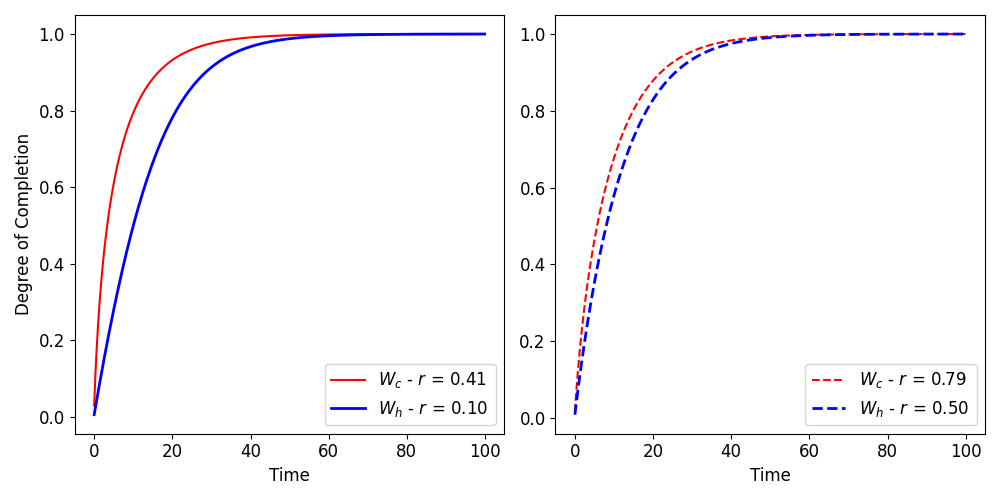
\includegraphics[width=0.7\linewidth]{Images/Gaussian/completion-squeezing.png}
    \caption{Degree of completion for a squeezed thermal state, with the right graph using a bigger squeezing parameter than the left graph.}
    \label{fig:completion-squeezing}
\end{figure}

\noindent From this expression, we can notice that squeezing thermal states with different temperatures do not preserve their equidistance, unlike the displacement operation case. As a consequence, in order to make a fair comparison, we must start with two equidistant squeezed states. The ergotropy of a squeezed thermal state is
\begin{equation}
    \mathcal{E}(t) = \omega f(\beta_t) (\cosh (2r_t) - 1).
    \label{eq:ergo-squeezing}
\end{equation}

\noindent Because of the dependence of $f(\beta_t)$, applying the same squeezing (that is, the same $r_t$ and $\phi_t$) in different thermal states results in a higher ergotropy to the squeezed hotter state. Therefore, to make an even fairer comparison, we will impose that the initial states must have the same initial ergotropy.

The Wigner-Fisher Information of a squeezed thermal state is
\begin{equation}
    I_W (t) = 2 \dot{S}_W^2 + 8 \dot{r}_t^2 + 2 \dot{\phi}_t^2 \sinh^2 (2r_t).
    \label{eq:Iw-squeezing}
\end{equation}

\noindent Again, obtaining analytical thermal kinematic expressions from Eq. \eqref{eq:Iw-squeezing} will not bring additional information, so we will solve it numerically. From the degree of completion (Fig. \ref{fig:completion-squeezing}), the thermal relaxation of $W_c$ is still faster than that of $W_h$, like in Secs. \eqref{sec:result-thermal} and \eqref{sec:result-displaced}. However, increasing the squeezing parameter reduces the asymmetry.

To understand why the asymmetry is reduced for the case with a bigger squeezing parameter, we can analyse the entropy production rate. Fig. \ref{fig:contribution-small-squeezing} corresponds to a smaller $r$ and Fig. \ref{fig:contribution-big-squeezing} corresponds to a bigger $r$. Each graph shows the total entropy production rate (solid line) with its passive (dashed line) and ergotropic (dotted line) contributions. Unlike the displacement operation, the squeezing change affects both passive and ergotropic contributions.

\begin{figure}[b!]
    \centering
    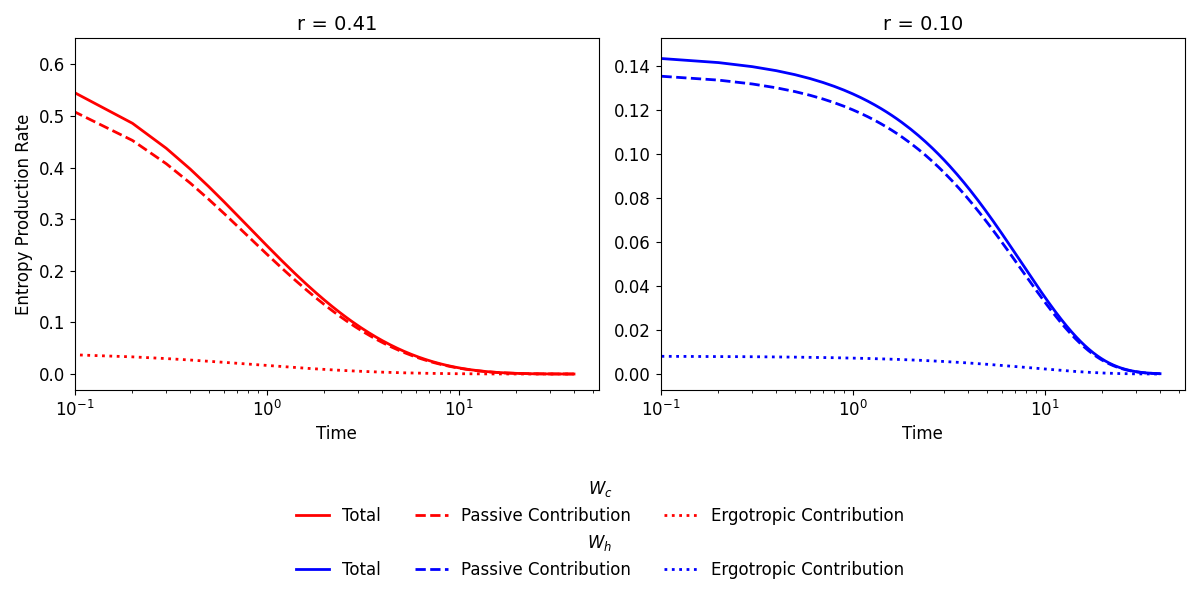
\includegraphics[width=0.8\linewidth]{Images/Gaussian/Sprod-contribution1-squeezing.png}
    \caption{Entropy production rate for heating (red) and cooling (blue) weakly squeezed thermal state. There are the passive contribution (dashed) and ergotropic contribution (dotted) of the total entropy production rate (solid).}
    \label{fig:contribution-small-squeezing}
\end{figure}

\begin{figure}[t]
    \centering
    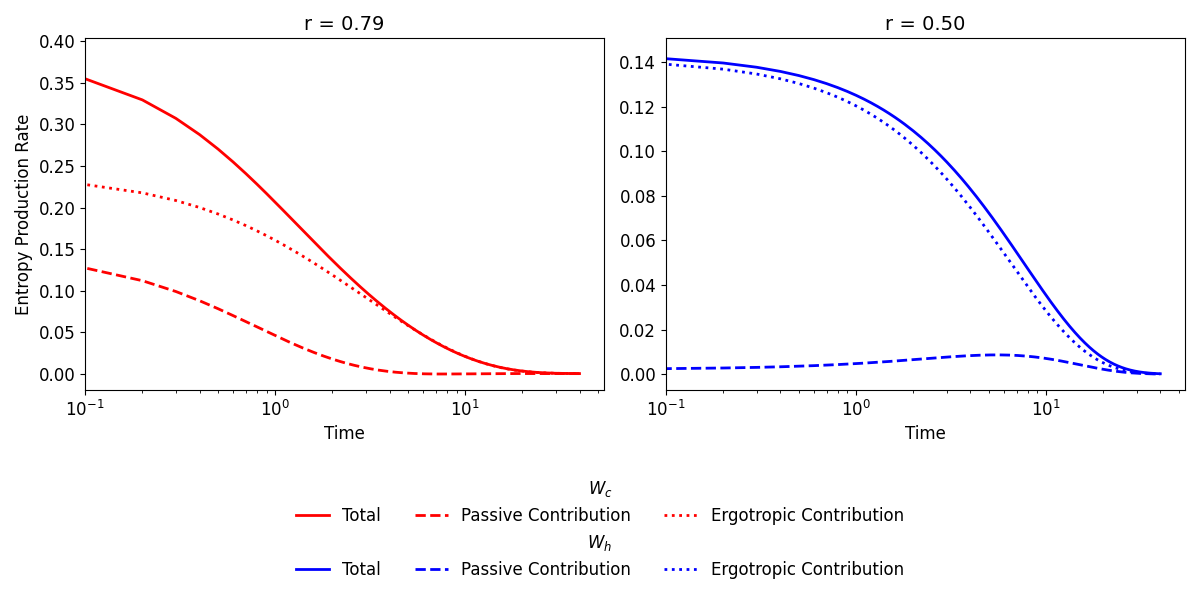
\includegraphics[width=0.8\linewidth]{Images/Gaussian/Sprod-contribution2-squeezing.png}
    \caption{Entropy production rate for heating (red) and cooling (blue) strongly squeezed thermal states. There are the passive contribution (dashed) and ergotropic contribution (dotted) of the total entropy production rate (solid).}
    \label{fig:contribution-big-squeezing}
\end{figure}


\subsubsection{Heating a displaced state and cooling a squeezed state}\label{sec:result-invertion}

After comparing the thermal relaxation of states with the same quantum resource, this section studies the behaviour of the asymmetry when applying different quantum resources to each initial state. Let's apply the displacement on the colder state and the squeezing on the hotter state. The initial states must have the same initial Wigner relative entropy, that is, $K[W_d || W_f] = K[W_s || W_f]$, and the same initial ergotropy, $\mathcal{E}_d = \mathcal{E}_s$.

\begin{figure}[b!]
    \centering
    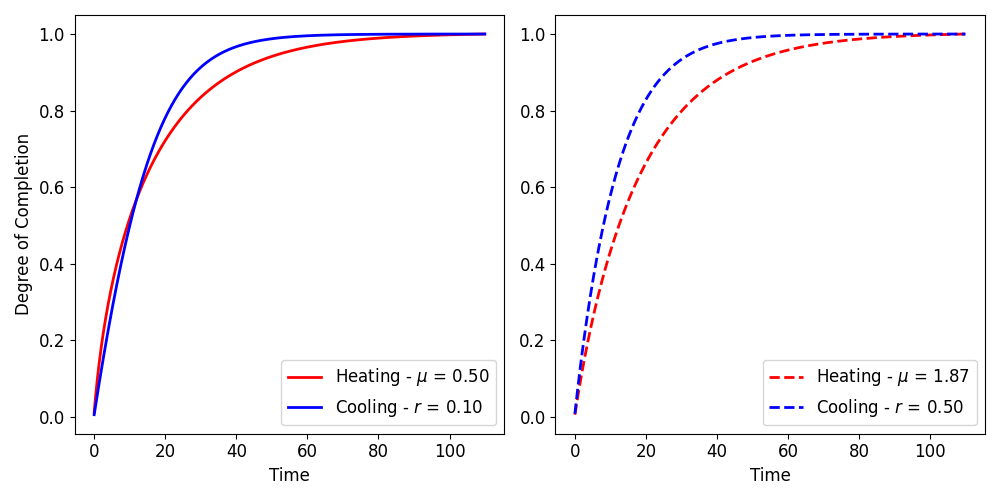
\includegraphics[width=0.8\linewidth]{Images/Gaussian/completion-invertion.png}
    \caption{Degree of completion for heating (red) a displaced thermal state and cooling (blue) a squeezed thermal state.}
    \label{fig:completion-inversion}
\end{figure}

The degree of completion for this system is presented in Fig. \ref{fig:completion-inversion}, and shows that it is possible to invert the asymmetry depending on the initial state condition. In the left graph, the displacement and squeezing parameters are smaller than in the right graph, and the asymmetry inversion is partial because cooling is faster only in some period of time. In the right graph, where the parameters are bigger, cooling is faster than heating for all times.

To study the entropy production rate of heating, we used the same expressions of Section \ref{sec:result-displaced}, and for the entropy production rate of cooling, we used the expressions of Section \ref{sec:result-squeezed}. Fig. \ref{fig:sprod-inversion-small} and Fig. \ref{fig:sprod-inversion-big} show the ergotropic and passive contributions for the entropy production of smaller and bigger parameters, respectively. The comparison of these graphs indicates that cooling becomes completely faster than heating only when its entropy production is initially higher.

\begin{figure}[b!]
    \centering
    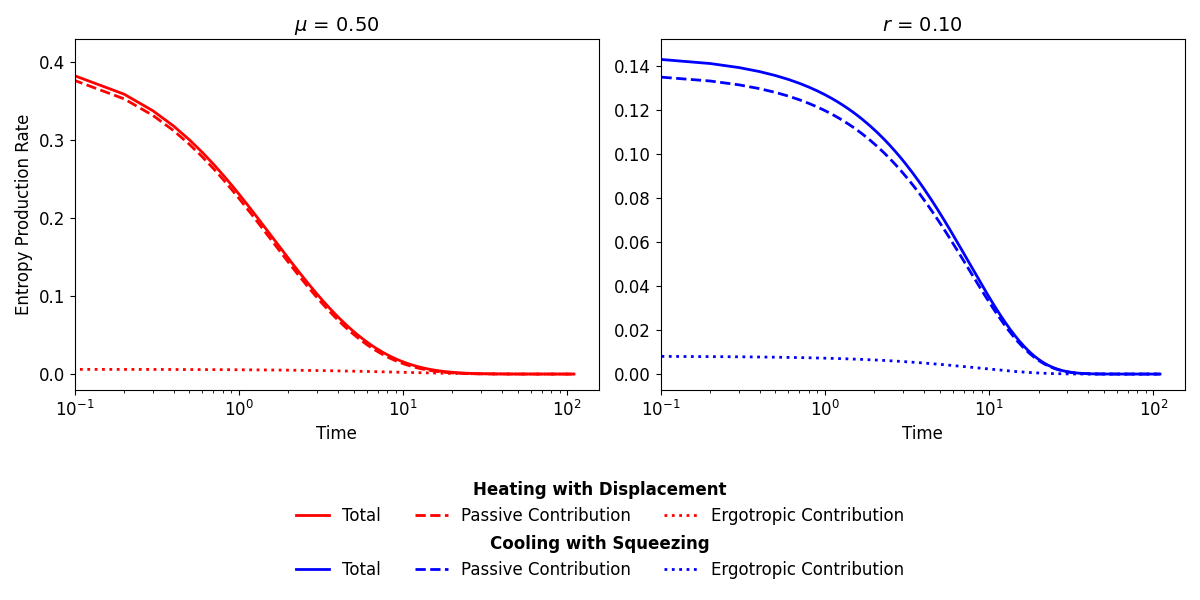
\includegraphics[width=0.8\linewidth]{Images/Gaussian/contributions-small-invertion.png}
    \caption{Entropy production rate for heating (red) a state with small $\mu$ and cooling (blue) a state with small $r$. The passive contribution is in dashed lines, the ergotropic contribution is in dotted lines, and the total entropy production rate is in solid lines.}
    \label{fig:sprod-inversion-small}
\end{figure}

\begin{figure}[b!]
    \centering
    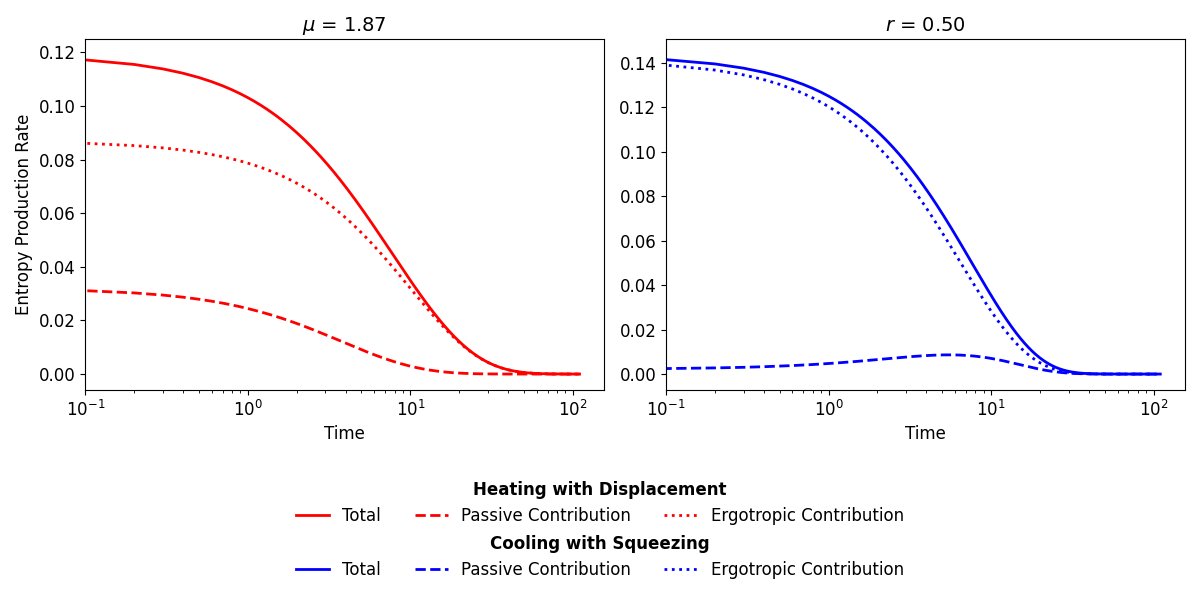
\includegraphics[width=0.8\linewidth]{Images/Gaussian/contributions-big-inversion.png}
    \caption{Entropy production rate for heating (red) a state with big $\mu$ and cooling (blue) a state with big $r$. The passive contribution is in dashed lines, the ergotropic contribution is in dotted lines, and the total entropy production rate is in solid lines.}
    \label{fig:sprod-inversion-big}
\end{figure}

%% USPSC-Cap3-Conclusao.tex
% ---
% Conclusão
% ---
\chapter{Conclusão}\label{cap:conclusion}



% ----------------------------------------------------------
% ELEMENTOS PÓS-TEXTUAIS
% ----------------------------------------------------------
\postextual

% Referências bibliográficas
\bibliography{USPSC-bib/USPSC-modelo-references}

% Apêndices e Anexos
%% USPSC-Apendice.tex
% ---
% Inicia os apêndices
% ---

\begin{apendicesenv}

\chapter{Concurrence of an X-state}
\label{apx:concurrence}

A general way to define an X-state is
\begin{equation}
    \rho = 
    \begin{bmatrix}
        a & 0 & 0 & f\\
        0 & b & e & 0\\
        0 & e^* & c & 0\\
        f^* & 0 & 0 & d
    \end{bmatrix}.
\end{equation}

\noindent As we presented in Sec. \ref{sec:correlations}, the concurrence of two qubits is defined as
\begin{equation}
    C({\rho}) = \max\{ 0, \lambda_1 - \lambda_2 - \lambda_3 - \lambda_4 \},
\end{equation}

\noindent where $\lambda_i > \lambda_j$ for $i<j$ are the square root of the eigenvalues of the matrix $R = \rho \tilde{\rho}$ with $\tilde{\rho} = (\sigma_y \otimes \sigma_y) \rho^* (\sigma_y \otimes \sigma_y)$ and $\rho^*$ being the complex conjugate of the density matrix. To start computing the concurrence of an X-state, we first find that
\begin{equation}
    \rho^* = 
    \begin{bmatrix}
        a & 0 & 0 & f^*\\
        0 & b & e^* & 0\\
        0 & e & c & 0\\
        f & 0 & 0 & d
    \end{bmatrix}.
\end{equation}

\noindent Using that
\begin{equation}
    \sigma_y \otimes \sigma_y = 
    \begin{bmatrix}
        0 & -i\\
        i & 0
    \end{bmatrix} \otimes
    \begin{bmatrix}
        0 & -i\\
        i & 0
    \end{bmatrix} =
    \begin{bmatrix}
        0 & 0 & 0 & -1\\
        0 & 0 & 1 & 0\\
        0 & 1 & 0 & 0\\
        -1 & 0 & 0 & 1
    \end{bmatrix},
\end{equation}

\noindent it is possible to compute
\begin{equation}
    \begin{split}
        \tilde{\rho} &= (\sigma_y \otimes \sigma_y) \rho^* (\sigma_y \otimes \sigma_y)\\
        &= \begin{bmatrix}
        0 & 0 & 0 & -1\\
        0 & 0 & 1 & 0\\
        0 & 1 & 0 & 0\\
        -1 & 0 & 0 & 1
    \end{bmatrix}
    \begin{bmatrix}
        a & 0 & 0 & f^*\\
        0 & b & e^* & 0\\
        0 & e & c & 0\\
        f & 0 & 0 & d
    \end{bmatrix}
    \begin{bmatrix}
        0 & 0 & 0 & -1\\
        0 & 0 & 1 & 0\\
        0 & 1 & 0 & 0\\
        -1 & 0 & 0 & 1
    \end{bmatrix}\\
    &= \begin{bmatrix}
        d & 0 & 0 & f\\
        0 & c & e & 0\\
        0 & e^* & b & 0\\
        f^* & 0 & 0 & a
    \end{bmatrix}.
    \end{split}
\end{equation}

\noindent As a result, we find
\begin{equation}
    \begin{split}
        R &= \rho \tilde{\rho}\\
        &= \begin{bmatrix}
        a & 0 & 0 & f\\
        0 & b & e & 0\\
        0 & e^* & c & 0\\
        f^* & 0 & 0 & d
    \end{bmatrix}
    \begin{bmatrix}
        d & 0 & 0 & f\\
        0 & c & e & 0\\
        0 & e^* & b & 0\\
        f^* & 0 & 0 & a
    \end{bmatrix}\\
    &= \begin{bmatrix}
        ad+|f|^2 & 0 & 0 & 2af\\
        0 & bc+|e|^2 & 2be & 0\\
        0 & 2ce^* & bc+|e|^2 & 0\\
        2df^* & 0 & 0 & ad+|f|^2
    \end{bmatrix}.
    \end{split}
\end{equation}

\noindent To obtain the concurrence, we must use the eigenvalues of $R$: $\lambda_1 = ad+|f|^2 (1 + 2\sqrt{ad})$, $\lambda_2 = ad+|f|^2 (1 - 2\sqrt{ad})$, $\lambda_3 =  bc+|e|^2(1 + 2\sqrt{bc})$, and $\lambda_4 =  bc+|e|^2(1 - 2\sqrt{bc})$. Without specifying the matrix elements of $\rho$, we cannot go further. But the next steps are taking the square root of each eigenvalue of $R$, organizing them in decreasing order and substituting in Eq. \eqref{eq:concurrence}.




%%%%%%%%%%%%%%%%%%%%%%%%%%%%%%%%%%%%%%%%%%%%%%%%%%%%%
\chapter{Derivation of the Wigner-Fisher information}
\label{apx:WFI}

The Wigner-Fisher information can be obtained from similar calculations as the ones of Sec \ref{sec:thermal-kinematics}. First, we consider two close Wigner distributions and make a second order Taylor expansion in a parameter $\theta$ of $W(\mathbf{x}, \theta+d\theta)$, finding that the Wigner relative entropy (defined in the first equality of Eq. \eqref{eq:wigner-relative-entropy}) becomes
\begin{equation}
    \begin{split}
        K[&W(\mathbf{x}, \theta+d\theta) || W(\mathbf{x}, \theta)] = \int W(\mathbf{x}, \theta+d\theta) \ln \left ( \frac{W(\mathbf{x}, \theta+d\theta)}{W(\mathbf{x}, \theta)} \right ) d^2 \mathbf{x} \\
        &= \int [W(\mathbf{x}, \theta) + \partial_\theta W(\mathbf{x}, \theta) d\theta + \frac{1}{2} \partial_\theta^2 W(\mathbf{x}, \theta) d\theta^2 + \mathcal{O}(d\theta^3)]\\
        &\times \left[\frac{\partial_\theta W(\mathbf{x}, \theta)}{W(\mathbf{x}, \theta)} d\theta + \frac{1}{2}\frac{\partial_\theta^2 W(\mathbf{x}, \theta)}{W(\mathbf{x}, \theta)} d\theta^2 - \frac{1}{2} \frac{(\partial_\theta W(\mathbf{x}, \theta)d\theta)^2}{W(\mathbf{x}, \theta)^2} + \mathcal{O}(d\theta^3) \right] d^2 \mathbf{x} \\
        &= \frac{1}{2}\int \frac{(\partial_\theta W(\mathbf{x}, \theta) d\theta)^2}{W(\mathbf{x}, \theta)} d^2 \mathbf{x} + \mathcal{O}(d\theta^3)\\
        &= \frac{1}{2} \mathcal{I}_W(\theta) d\theta^2 + \mathcal{O}(d\theta^3),
    \end{split}
\end{equation}

\noindent where we used $\ln (1+x) = x - \frac{1}{2}x^2 + \mathcal{O}(x^3)$ in the second line and that $\int W(\mathbf{x}, \theta) d^2 \mathbf{x} = 1$ in the third line. In the last equality, we identify the Wigner-Fisher information as 
\begin{equation}
    \mathcal{I}_W(\theta) = \int \frac{(\partial_\theta W(\mathbf{x}, \theta) d\theta)^2}{W(\mathbf{x}, \theta)}.
\end{equation}

\noindent Additionally, we can also write the Wigner-Fisher information in terms of the mean vector and the covariance matrix. One way to do it, is expanding the last line of Eq. \eqref{eq:wigner-relative-entropy}, that in our case is
\begin{equation}
    \begin{split}
        K[W(\mathbf{x}, \theta+d\theta) || W(\mathbf{x}, \theta)] &= -1 + \frac{1}{2} \Big[(\mathbf{v}_{\theta+d\theta} - \mathbf{v}_\theta)^\dagger \Theta_\theta^{-1} (\mathbf{v}_{\theta+d\theta} - \mathbf{v}_\theta) \\
        &+ \text{Tr}(\Theta_\theta^{-1} \Theta_{\theta+d\theta}) + \ln \frac{|\Theta_\theta|}{|\Theta_{\theta+d\theta}|} \Big].
    \end{split}
    \label{eq:K-wigner-fisher}
\end{equation}

\noindent First, we use the second order Taylor expansion of
\begin{align}
    &\mathbf{v}_{\theta+d\theta} \approx \mathbf{v}_{\theta} + \left(\frac{d\mathbf{v}_{\theta}}{d\theta}\right)d\theta + \frac{1}{2}\left(\frac{d^2\mathbf{v}_{\theta}}{d\theta^2}\right)d\theta^2 , \\
    &\Theta_{\theta+d\theta} \approx \Theta_{\theta} + \left(\frac{d\Theta_{\theta}}{d\theta}\right)d\theta + \frac{1}{2}\left(\frac{d^2\Theta_{\theta}}{d\theta^2}\right)d\theta^2 , \\
    &\ln( |\Theta_{\theta+d\theta}|) \approx \ln( |\Theta_{\theta}|) + \left(\frac{d}{d\theta} \ln( |\Theta_{\theta}|)\right)d\theta + \frac{1}{2}\left(\frac{d^2}{d\theta^2} \ln( |\Theta_{\theta}|) \right)d\theta^2,
    \label{eq:expansao-ln-Theta}
\end{align}

\noindent such that the mean vector term in Eq. \eqref{eq:K-wigner-fisher} becomes
\begin{equation}
    (\mathbf{v}_{\theta+d\theta} - \mathbf{v}_\theta)^\dagger \Theta_\theta^{-1} (\mathbf{v}_{\theta+d\theta} - \mathbf{v}_\theta) \approx \dot{\mathbf{v}}_{\theta}^\dagger \Theta_\theta^{-1} \dot{\mathbf{v}}_{\theta} d\theta^2,
\end{equation}

\noindent and the trace term in Eq. \eqref{eq:K-wigner-fisher} becomes
\begin{align}
    \text{Tr}(\Theta_\theta^{-1} \Theta_{\theta+d\theta}) &\approx \text{Tr}\left[\Theta_\theta^{-1} \Theta_{\theta} + \Theta_\theta^{-1} \dot{\Theta}_{\theta} d\theta + \frac{1}{2} \Theta_\theta^{-1} \ddot{\Theta}_{\theta} d\theta^2 \right] \nonumber\\
    &= 2 + \text{Tr}\left[\Theta_\theta^{-1} \dot{\Theta}_{\theta} \right] d\theta + \frac{1}{2} \text{Tr}\left[\Theta_\theta^{-1} \ddot{\Theta}_{\theta} \right] d\theta^2.
\end{align}

\noindent To rewrite the logarithm term in Eq. \eqref{eq:K-wigner-fisher}, we will need the identities \cite{medina-2026}
\begin{align}
    &\frac{d}{d\theta} \ln(|\Theta_\theta|) = \text{Tr}\left[\Theta_\theta^{-1} \dot{\Theta}_{\theta} \right]\\
    &\frac{d^2}{d\theta^2} \ln(|\Theta_\theta|) = \text{Tr}\left[\Theta_\theta^{-1} \ddot{\Theta}_{\theta} + \Theta_\theta^{-1} \dot{\Theta}_{\theta}\Theta_\theta^{-1} \dot{\Theta}_{\theta} \right],
\end{align}

\noindent which can be used in Eq. \eqref{eq:expansao-ln-Theta}, resulting in
\begin{equation}
    \ln( |\Theta_{\theta+d\theta}|) \approx \ln( |\Theta_{\theta}|) + \text{Tr}\left[\Theta_\theta^{-1} \dot{\Theta}_{\theta} \right] d\theta + \frac{1}{2}\text{Tr}\left[\Theta_\theta^{-1} \ddot{\Theta}_{\theta} + \Theta_\theta^{-1} \dot{\Theta}_{\theta}\Theta_\theta^{-1} \dot{\Theta}_{\theta} \right]d\theta^2,
\end{equation}

\noindent that allow us to rewrite the logarithm term as
\begin{equation}
    \ln \frac{|\Theta_\theta|}{|\Theta_{\theta+d\theta}|} \approx -\text{Tr}\left[\Theta_\theta^{-1} \dot{\Theta}_{\theta} \right] d\theta - \frac{1}{2}\text{Tr}\left[\Theta_\theta^{-1} \ddot{\Theta}_{\theta}\right]d\theta^2 + \text{Tr}\left[(\Theta_\theta^{-1} \dot{\Theta}_{\theta})^2 \right]d\theta^2.
\end{equation}

\noindent As a result, the Wigner relative entropy expanded in terms of the mean vector and covariance matrix is
\begin{equation}
    K[W(\mathbf{x}, \theta+d\theta) || W(\mathbf{x}, \theta)] \approx \frac{1}{2} \{\dot{\mathbf{v}}_t^\dagger \Theta^{-1}_t \dot{\mathbf{v}}_t + \text{Tr}[(\Theta_t^{-1} \dot{\Theta}_t)^2]\} d\theta^2,
\end{equation}

\noindent in which we identify the Wigner-Fisher information as
\begin{equation}
    \mathcal{I}_W (t) = \dot{\mathbf{v}}_t^\dagger \Theta^{-1}_t \dot{\mathbf{v}}_t + \text{Tr}[(\Theta_t^{-1} \dot{\Theta}_t)^2].
\end{equation}

\end{apendicesenv}
% ---
\include{USPSC-TA-PosTextual/USPSC-Anexos}

% Índice Remissivo
\include{USPSC-IndicesRemissivos}

\end{document}
